% Options for packages loaded elsewhere
\PassOptionsToPackage{unicode}{hyperref}
\PassOptionsToPackage{hyphens}{url}
\PassOptionsToPackage{dvipsnames,svgnames,x11names}{xcolor}
%
\documentclass[
  letterpaper,
  DIV=11,
  numbers=noendperiod]{scrreprt}

\usepackage{amsmath,amssymb}
\usepackage{lmodern}
\usepackage{iftex}
\ifPDFTeX
  \usepackage[T1]{fontenc}
  \usepackage[utf8]{inputenc}
  \usepackage{textcomp} % provide euro and other symbols
\else % if luatex or xetex
  \usepackage{unicode-math}
  \defaultfontfeatures{Scale=MatchLowercase}
  \defaultfontfeatures[\rmfamily]{Ligatures=TeX,Scale=1}
\fi
% Use upquote if available, for straight quotes in verbatim environments
\IfFileExists{upquote.sty}{\usepackage{upquote}}{}
\IfFileExists{microtype.sty}{% use microtype if available
  \usepackage[]{microtype}
  \UseMicrotypeSet[protrusion]{basicmath} % disable protrusion for tt fonts
}{}
\makeatletter
\@ifundefined{KOMAClassName}{% if non-KOMA class
  \IfFileExists{parskip.sty}{%
    \usepackage{parskip}
  }{% else
    \setlength{\parindent}{0pt}
    \setlength{\parskip}{6pt plus 2pt minus 1pt}}
}{% if KOMA class
  \KOMAoptions{parskip=half}}
\makeatother
\usepackage{xcolor}
\setlength{\emergencystretch}{3em} % prevent overfull lines
\setcounter{secnumdepth}{0}
% Make \paragraph and \subparagraph free-standing
\ifx\paragraph\undefined\else
  \let\oldparagraph\paragraph
  \renewcommand{\paragraph}[1]{\oldparagraph{#1}\mbox{}}
\fi
\ifx\subparagraph\undefined\else
  \let\oldsubparagraph\subparagraph
  \renewcommand{\subparagraph}[1]{\oldsubparagraph{#1}\mbox{}}
\fi


\providecommand{\tightlist}{%
  \setlength{\itemsep}{0pt}\setlength{\parskip}{0pt}}\usepackage{longtable,booktabs,array}
\usepackage{calc} % for calculating minipage widths
% Correct order of tables after \paragraph or \subparagraph
\usepackage{etoolbox}
\makeatletter
\patchcmd\longtable{\par}{\if@noskipsec\mbox{}\fi\par}{}{}
\makeatother
% Allow footnotes in longtable head/foot
\IfFileExists{footnotehyper.sty}{\usepackage{footnotehyper}}{\usepackage{footnote}}
\makesavenoteenv{longtable}
\usepackage{graphicx}
\makeatletter
\def\maxwidth{\ifdim\Gin@nat@width>\linewidth\linewidth\else\Gin@nat@width\fi}
\def\maxheight{\ifdim\Gin@nat@height>\textheight\textheight\else\Gin@nat@height\fi}
\makeatother
% Scale images if necessary, so that they will not overflow the page
% margins by default, and it is still possible to overwrite the defaults
% using explicit options in \includegraphics[width, height, ...]{}
\setkeys{Gin}{width=\maxwidth,height=\maxheight,keepaspectratio}
% Set default figure placement to htbp
\makeatletter
\def\fps@figure{htbp}
\makeatother

\KOMAoption{captions}{tableheading}
\makeatletter
\makeatother
\makeatletter
\@ifpackageloaded{bookmark}{}{\usepackage{bookmark}}
\makeatother
\makeatletter
\@ifpackageloaded{caption}{}{\usepackage{caption}}
\AtBeginDocument{%
\ifdefined\contentsname
  \renewcommand*\contentsname{Table of contents}
\else
  \newcommand\contentsname{Table of contents}
\fi
\ifdefined\listfigurename
  \renewcommand*\listfigurename{List of Figures}
\else
  \newcommand\listfigurename{List of Figures}
\fi
\ifdefined\listtablename
  \renewcommand*\listtablename{List of Tables}
\else
  \newcommand\listtablename{List of Tables}
\fi
\ifdefined\figurename
  \renewcommand*\figurename{Figure}
\else
  \newcommand\figurename{Figure}
\fi
\ifdefined\tablename
  \renewcommand*\tablename{Table}
\else
  \newcommand\tablename{Table}
\fi
}
\@ifpackageloaded{float}{}{\usepackage{float}}
\floatstyle{ruled}
\@ifundefined{c@chapter}{\newfloat{codelisting}{h}{lop}}{\newfloat{codelisting}{h}{lop}[chapter]}
\floatname{codelisting}{Listing}
\newcommand*\listoflistings{\listof{codelisting}{List of Listings}}
\makeatother
\makeatletter
\@ifpackageloaded{caption}{}{\usepackage{caption}}
\@ifpackageloaded{subcaption}{}{\usepackage{subcaption}}
\makeatother
\makeatletter
\@ifpackageloaded{tcolorbox}{}{\usepackage[many]{tcolorbox}}
\makeatother
\makeatletter
\@ifundefined{shadecolor}{\definecolor{shadecolor}{rgb}{.97, .97, .97}}
\makeatother
\makeatletter
\makeatother
\ifLuaTeX
  \usepackage{selnolig}  % disable illegal ligatures
\fi
\IfFileExists{bookmark.sty}{\usepackage{bookmark}}{\usepackage{hyperref}}
\IfFileExists{xurl.sty}{\usepackage{xurl}}{} % add URL line breaks if available
\urlstyle{same} % disable monospaced font for URLs
\hypersetup{
  pdftitle={Solucionaro de Control Automático de Procesos},
  pdfauthor={Ever Vino},
  colorlinks=true,
  linkcolor={blue},
  filecolor={Maroon},
  citecolor={Blue},
  urlcolor={Blue},
  pdfcreator={LaTeX via pandoc}}

\title{Solucionaro de Control Automático de Procesos}
\author{Ever Vino}
\date{9/1/23}

\begin{document}
\maketitle
\ifdefined\Shaded\renewenvironment{Shaded}{\begin{tcolorbox}[sharp corners, boxrule=0pt, breakable, enhanced, borderline west={3pt}{0pt}{shadecolor}, interior hidden, frame hidden]}{\end{tcolorbox}}\fi

\bookmarksetup{startatroot}

\hypertarget{un-solucionario-para-control-automuxe1tico}{%
\chapter*{Un solucionario para Control
Automático}\label{un-solucionario-para-control-automuxe1tico}}
\addcontentsline{toc}{chapter}{Un solucionario para Control Automático}

\markboth{Un solucionario para Control Automático}{Un solucionario para
Control Automático}

Este es un Solucionario de Control Automático

\part{Sistemas físicos de primer orden}

\hypertarget{un-calentador-que-deja-de-funcionar}{%
\chapter{Un calentador que deja de
funcionar}\label{un-calentador-que-deja-de-funcionar}}

\hypertarget{problema-5.1-process-dynamics-modelling-and-control---babatunde-harmon}{%
\section*{Problema 5.1 (Process Dynamics, Modelling and Control -
Babatunde,
Harmon)}\label{problema-5.1-process-dynamics-modelling-and-control---babatunde-harmon}}
\addcontentsline{toc}{section}{Problema 5.1 (Process Dynamics, Modelling
and Control - Babatunde, Harmon)}

\markright{Problema 5.1 (Process Dynamics, Modelling and Control -
Babatunde, Harmon)}

\begin{figure}

{\centering 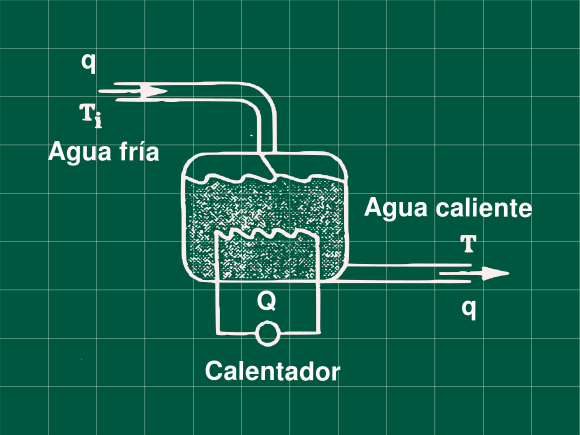
\includegraphics{././images/p5.1-babatunde/headercontrol51.png}

}

\caption{Sistema de calentador de agua}

\end{figure}

Para el proceso mostrado en la figura, un calentador electrico de agua.
En un día particular el tanque trabajaba a temperatura de 80 °C, y de
repente el calentador se rompe y dejar de suministrar calor, a este
tiempo el tanque con 100 L de capacidad operaba con un caudal 10 L/min,
la temperatura del agua fria es de 30 °C. Esto pasa durante 5 minutos,
luego el calentador detiene el flujo de agua(debido al diseño del
calentador). Desarrolle un apropiado modelo matemático para este
proceso, y resolviendo la ecuación diferencial encuentre la temperatura
del tanque a los 5 minutos

\hypertarget{resoluciuxf3n}{%
\section{Resolución}\label{resoluciuxf3n}}

Escribiendo nuestro balance de energía

\[
\rho C_p V \frac{dT}{dt}=q \rho C_p(T_i-T)+Q\space\space\space\textbf{ .... (1)}
\]

Balance en estado estacionario

\[
0 = q \rho C_p(T_{is}-T_s)+Q_s\space\space\space\textbf{ .... (2)}
\]

Calculamos la ecuación (2) el valor de \(Q_s\) que nos a servir luego

\[
0 = q \rho C_p(30-80)+Q_s
\]

\[
Q_s=50q\rho C_p
\]

Restando (1) con (2) y tranformando a variables desviación

\[
\rho C_p V \frac{d(T-T_s)}{dt}=q \rho C_p\big[(T_i-T_{is})-(T-T_s)\big]+Q-Q_s
\]

\[
\rho C_p V \frac{dT'}{dt}=q \rho C_p\big[T'_i-T'\big]+Q'
\]

Aplicando la transformada de Laplace y despejando la función
transferencia

\[
\rho C_p V sT'(s)=q \rho C_p\big[T'_i(s)-T'(s)\big]+Q'(s)
\]

\[
\frac{T'(s)}{Q'(s)}=\frac{1}{V\rho C_p s+q\rho C_p}\space\space\space\textbf{ .... (3)}
\]

Describimos la perturbación del enunciado sabemos que el calor
suministrado baja cero cuando t\textgreater0.

\[
Q'(t)= Q(t)-Q_s
\begin{cases}
   Q_s-Q_s &\text{si } t < 0 \\
   0 - Q_s &\text{si } t > 0\\
\end{cases}
\]

\[
Q'(t)=
\begin{cases}
   &\text{si } t < 0 \\
   - Q_s &\text{si } t > 0\\
\end{cases}
\]

\[
Q'(t) = -Q_s
\]

Aplicando al transformada de Laplace

\[
Q'(s)= -\frac{Q_s}{s}
\]

Reemplazando en la ecuacion (3) y sabiendo que \(Q_s=50q\rho C_p\)

\[
T'(s)=-\frac{50q\rho C_p}{s(V\rho C_p s+q\rho C_p)}
\]

Operando y reemplazando valores conocidos \(V=100\) y \(q=10\)

\[
T'(s)=-\frac{50}{s(Vs+q)}=-\frac{50}{s(10s+1)}
\]

Antitransformando, recuerde \(T'(t) = T(t)-T_s\)

\[
T'(t)=50(e^{-t/10}-1)
\]

\[
T(t)=50(e^{-t/10}-1)+80
\]

Hallando la temperatura a t = 5 min \[
T(t=5)=50(e^{-5/10}-1)+80
\]

\[
\mathbf{T(t=5min)=60.33\ °C}
\]

\hypertarget{referencias}{%
\section{Referencias}\label{referencias}}

\begin{itemize}
\tightlist
\item
  Babatunde, A. O.; Harmon, W. R. (1994). \emph{process dynamics,
  modeling, and control}. OXFORD UNIVERSITY PRESS. ISBN 0-19-509119-1
\end{itemize}

\hypertarget{un-sistema-con-un-tanque-una-bomba-y-una-vuxe1lvula}{%
\chapter{Un sistema con un tanque, una bomba y una
válvula}\label{un-sistema-con-un-tanque-una-bomba-y-una-vuxe1lvula}}

\begin{figure}

{\centering 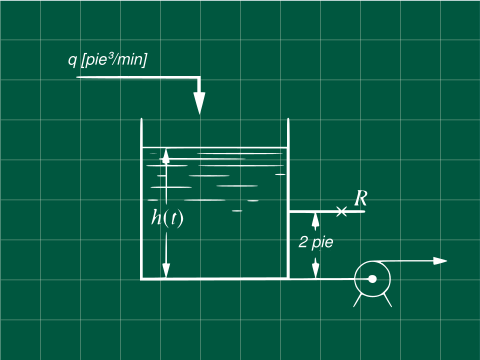
\includegraphics{././images/p5.1-coughanowr/headercontrol.png}

}

\caption{Grafico de prob 5.1}

\end{figure}

Derive la ecuación transferencia H(s)/Q(s) para el nivel del líquido del
sistema mostrado en la figura, cuando el tanque opera en estado
estacionario a:

\begin{itemize}
\item
  \begin{enumerate}
  \def\labelenumi{\alph{enumi})}
  \tightlist
  \item
    \(\text{  }h_s = 1 \text{ pie}\)
  \end{enumerate}
\item
  \begin{enumerate}
  \def\labelenumi{\alph{enumi})}
  \setcounter{enumi}{1}
  \tightlist
  \item
    \(\text{  }h_s = 3 \text{ pie}\)
  \end{enumerate}
\end{itemize}

La bomba extrae agua a caudal constante de \(10\text{ pie³/min}\) y es
independiente del la altura \(h\), El área seccional es
\(A = 1.0\text{ pie²}\) y la resistencia es \(R=0.5\text{ pie³/min}\).

\hypertarget{resoluciuxf3n-1}{%
\section{Resolución}\label{resoluciuxf3n-1}}

\hypertarget{resolviendo-para-h_s1textpie}{%
\subsection{\texorpdfstring{Resolviendo para
\(h_s=1\text{pie}\)}{Resolviendo para h\_s=1\textbackslash text\{pie\}}}\label{resolviendo-para-h_s1textpie}}

Cuando la altura \(h_s=1\) podemos notar que no existe flujo posible por
la válvula, por lo que no lo consideramos en la ecuación transferencia.

Escribiendo las ecuaciones de balance

\[
q - q_b = \frac{dV}{dt} = A\frac{dh}{dt} \space\space\space\space\space \textbf{(1)}
\]

Ecuacion en estado estacionario

\[
q_s - q_b = 0 \space\space\space\space\space \textbf{(2)}
\]

Restando (1) con (2) para obtener las variables desviación y recordando
que \(dh=d(h-h_s)\), por ser \(h_s\) constante.

\[
q-q_s=A\frac{d(h-h_s)}{dt}
\]

\[
Q = A\frac{dH}{dt}
\]

Aplicando la tranformada de Laplace, sabiendo que
\(H(t=0)= h-h_s=h_s-h_s=0\) y \(A=1\text{ pie}\).

\[
Q(s)  = A(sH(s)-H(t=0))\\
\] \[
\mathbf{\frac{H(s)}{Q(s)}  = \frac{1}{s}}
\]

\hypertarget{resolviendo-para-h_s3text-pie}{%
\subsection{\texorpdfstring{Resolviendo para
\(h_s=3\text{ pie}\)}{Resolviendo para h\_s=3\textbackslash text\{ pie\}}}\label{resolviendo-para-h_s3text-pie}}

Cuando \(h_s=3\) el sistema se encuentra operando sobre el nivel de la
válvula, por lo que si existe un flujo \(q_0\) que pasa por este.

Aplicando un balance del sistema y sabiendo que \(q_0 = h-h_v/R\), donde
\(h_v\) es la altura de la válvula

\[
q - q_0- q_b = A\frac{dh}{dt}
\] \[
q - \frac{h-h_v}{R}- q_b = A\frac{dh}{dt} \space\space\space\space\space \textbf{(3)}
\]

Balance en estado estacionario

\[
q_s - \frac{h_s-h_v}{R}- q_b = 0 \space\space\space\space\space \textbf{(4)}
\]

Restando (3) con (4) para obtener las variables desviación y recordando
que \(dh=d(h-h_s)\), por ser \(h_s\) constante.

\[
q - q_s- \frac{h-h_s}{R} = A\frac{d(h-h_s)}{dt}
\]

\[
Q -\frac{H}{R} = A\frac{dH}{dt}
\]

Aplicando la tranformada de Laplace, sabiendo que
\(H(t=0)= h-h_s=h_s-h_s=0\), \(A=1\text{ pie}\) y
\(R=0.5\text{ pie/(pie³/min)}\).

\[
Q(s) -\frac{H(s)}{R} = A(sH(s)-H(t=0))\\
\] \[
\frac{H(s)}{Q(s)}  = \frac{R}{ARs+1}
\]

\[
\mathbf{\frac{H(s)}{Q(s)}  = \frac{0.5}{0.5s+1}}
\]

\hypertarget{referencias-1}{%
\section{Referencias}\label{referencias-1}}

\begin{itemize}
\tightlist
\item
  Coughanowr, D. R.; LeBlanc, S. E. (2009). \emph{Process Systems
  Analysis and Control} (3rd edition). McGraw-Hill. ISBN
  978-0-07-339789-4.
\end{itemize}

\hypertarget{un-tanque-con-una-bomba-y-una-vuxe1lvula-de-resistencia-variable}{%
\chapter{Un tanque con una bomba y una válvula de resistencia
variable}\label{un-tanque-con-una-bomba-y-una-vuxe1lvula-de-resistencia-variable}}

\begin{figure}

{\centering 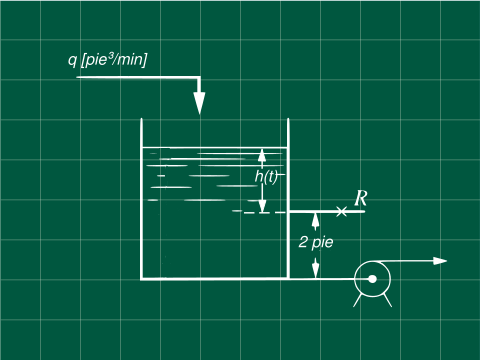
\includegraphics{././images/p5.2-coughanowr/headercontrol.png}

}

\caption{p5.9}

\end{figure}

El sistema mostrado en la figura tienen un área seccional
\(A=3\text{ pie²}\), la ecuación de la válvula es \(q=8\sqrt{h}\). Con q
en {[}pie³/min{]} y h (altura desde encima de la válvula) en {[}pie{]}.

Calcule la constante del tiempo \(\tau\) para cuando la altura por
encima de la válvula en estado estacionario es \textbf{a)} 3 pie y
\textbf{b)} 9 pie.

\hypertarget{resolviendo}{%
\subsection{Resolviendo}\label{resolviendo}}

\[
\begin{array}{l}
Datos\\
A = 3 \text{ pie²}\\
q_0=8 \sqrt{h}
\end{array}
\]

Linealizando \(q_0=8 \sqrt h\)

La expandimos usando las serie de Taylor al rededor del estado
estacionario.

\[
f(x) = f(x_s)+\frac{df}{dt}\bigg |_{x=x_s} (x-x_s)
\]

\[
q_0=8\sqrt{h_s}+\frac{4}{sqrt{h_s}}(h-hs)
\] \[
q_0=q_{0s}+\frac{4}{sqrt{h_s}}(h-hs)
\]

\[
q_0-q_{0s}=\frac{4}{\sqrt{h_s}}(h-hs)
\]

Hagamos \(R=\frac{\sqrt{h_s}}{4}\space\space\space\textbf{ (A)}\)

\[
q_0-q_{0s}=\frac{(h-hs)}{R}\space\space\space\space\textbf{(1)}
\]

Realizando el balance en el sistema

\[
q - q_0 - q_b= \frac{dV}{dt} \space\space\space\space (2)\textbf{(2)}
\]

Escribiendo el balance en estado estacionario

\[
q_s- q_s0 -q_b= 0 \space\space\space\space \textbf{(3)}
\]

Restando (2) con (1) para obtener las variables desviación y recordando
que \(dh=d(h-h_s)\), por ser \(h_s\) constante.

\[
q-q_s-(q_s-q_s0)=A\frac{d(h-h_s)}{dt}
\]

Reemplazando con la ecuación (1)

\[
q-q_s-\frac{(h-hs)}{R}=A\frac{d(h-h_s)}{dt}
\]

Transformando a variables desviación

\[
Q - \frac{H}{R} = A\frac{dH}{dt}
\]

Aplicando la tranformada de Laplace y sabiendo que
\(H(t=0)= h-h_s=h_s-h_s=0\)

\[
Q(s) - \frac{H(s)}{R} = A\left[sH(s)-H(t=0)\right]\\
\\
Q(s) - \frac{H(s)}{R} = AsH(s)
\]

\[
\frac{H(s)}{Q(s)}=\frac{R}{ARs+1} \\
\]

Por comparación con el modelo de primer orden
\(\frac{H(s)}{Q(s)}=\frac{Kp}{\tau s+1}\) y sabiendo que \(A=3\) y
\(R = \sqrt{h_s}/4\)

Notamos que \[\tau=AR=3\frac{\sqrt{h_s}}{4}\]

Para a) \(h_s=3\) \[
\mathbf{\tau = 1.2990\space min}
\] Para b) \(h_s=9\) \[
\mathbf{\tau = 2.25 \space min}
\]

\hypertarget{referencias-2}{%
\section{Referencias}\label{referencias-2}}

\begin{itemize}
\tightlist
\item
  Coughanowr, D. R.; LeBlanc, S. E. (2009). \emph{Process Systems
  Analysis and Control} (3rd edition). McGraw-Hill. ISBN
  978-0-07-339789-4.
\end{itemize}

\hypertarget{sistema-de-tanque-con-una-vuxe1lvula-de-resistencia-descrita-por-un-gruxe1fico}{%
\chapter{Sistema de tanque con una válvula de resistencia descrita por
un
gráfico}\label{sistema-de-tanque-con-una-vuxe1lvula-de-resistencia-descrita-por-un-gruxe1fico}}

\begin{figure}

{\centering 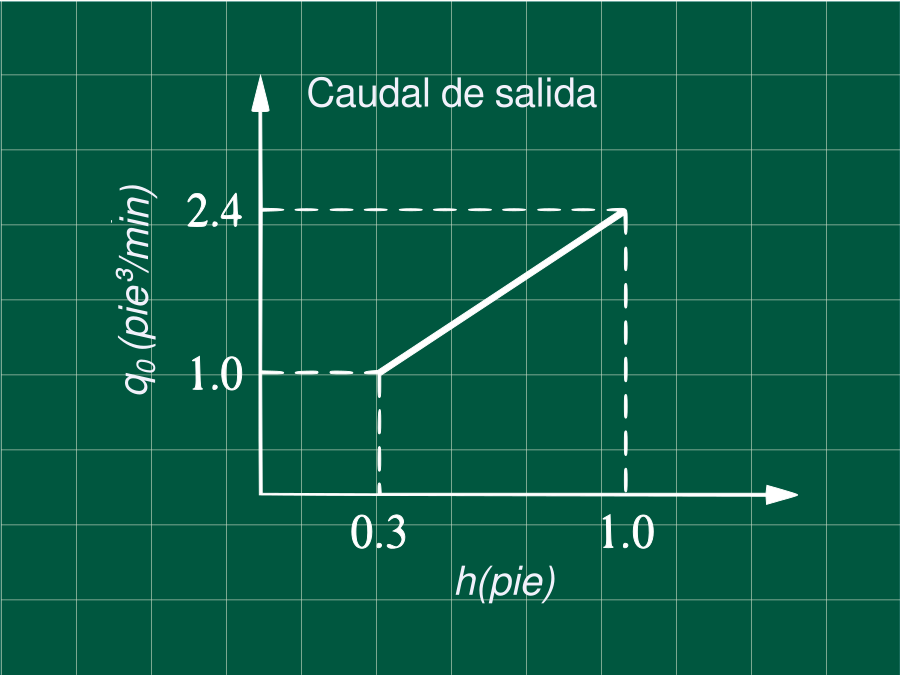
\includegraphics{././images/p5.3-coughanowr/headercontrol.png}

}

\caption{Grafico de prob 5.3}

\end{figure}

Un tanque con un área seccional de 2 pie² opera en estado estacionario
con un flujo de entrada de 2 pie³/min. El flujo de salida vs la altura
del sistema son representados en la figura.

Encuentre:

\begin{itemize}
\item
  La función transferencia \(H(s)/Q(s)\).
\item
  Si el flujo hacia el tanque se incrementa en de 2.0 a 2.2 pie³/min
  (paso unitario), calcule el nivel h, 2 minutos después del cambio.
\end{itemize}

\[
\begin{array}{l}
Datos\\
A = 2\space pie²\\
q_s = 2\space pie³/min
\end{array}
\]

\hypertarget{obtenciuxf3n-de-la-ecuaciuxf3n-q_0}{%
\subsection{\texorpdfstring{Obtención de la ecuación
\(q_0\)}{Obtención de la ecuación q\_0}}\label{obtenciuxf3n-de-la-ecuaciuxf3n-q_0}}

Como se observa en la gráfica \(q_0\) es función de la altura y es una
recta. Usando la fórmula de la ecuación de la recta que pasa por dos
puntos tenemos \((h_{1}=0.3,q_{01}=1)\) y \((h_{2}=1,q_{02}=2.4)\) :

\[
\frac{q_0-q_{01}}{h-h_1}=\frac{q_{02}-q_{01}}{h_2 - h_1}\\
\] \[
\frac{q_0-1}{h-0.3}=\frac{2.4-1}{1 - 0.3}\\
\] \[
q_0 = 2h+0.4
\]

Escribiendo las ecuaciones de balance \[
q - q_0 = \frac{dV}{dt}
\]

Pero \(q_0 = 2h+0.4\) y \(dV = Adh\)

\[
q- (2h+0.4) = A\frac{dh}{dt} \space\space\space\space (1)
\]

Escribiendo el balance en estado estacionario

\[
q_s- (2h_s+0.4) = 0 \space\space\space\space (2)
\]

Restando (1) con (2) para obtener las variables desviación y recordando
que \(dh=d(h-h_s)\), por ser \(h_s\) constante.

\[
q-q_s-2(h-h_s)+=A\frac{d(h-h_s)}{dt}
\]

\[
Q - 2\cdot H = A\frac{dH}{dt}
\]

Aplicando la tranformada de Laplacey sabiendo que
\(H(t=0)= h-h_s=h_s-h_s=0\)

\[
Q(s) - 2H(s) = A(sH(s)-H(t=0))\\
\] \[
Q(s) - 2H(s) = AsH(s)
\]

Despejando

\[
\mathbf{\frac{H(s)}{Q(s)}=\frac{1}{2 s+2}} \space\space\space\space (3) \\
\]

\hypertarget{descripciuxf3n-de-la-perturbaciuxf3n}{%
\subsection{Descripción de la
perturbación}\label{descripciuxf3n-de-la-perturbaciuxf3n}}

La perturbación sólo va a afectar el caudal de ingreso, esta puede ser
representado por la variable desviación \(Q(t)\)

\[
Q(t)=q-q_s=
\begin{cases}
   2.0-2.0 &\text{si } t < 0 \\
   2.2-2.0 \space\ pie³/min &\text{si } t>0\\
\end{cases}
\]

\[
Q(t)=
\begin{cases}
   0 &\text{si } t < 0 \\
   0.2 \space\ pie³/min &\text{si } t>0\\
\end{cases}
\]

Expresando la misma función con impulsos unitarios y aplicando la
transformada de Laplace

\[
Q(t) = 0.2\cdot u(t)
\] Entonces

\[
Q(s) = \frac{0.2}{s}
\]

\hypertarget{resolviendo-para-ht2}{%
\subsection{\texorpdfstring{Resolviendo para
\(h(t=2)\)}{Resolviendo para h(t=2)}}\label{resolviendo-para-ht2}}

Reemplazando la expresión anterior en la ecuación (3)

\[
\begin{array}{l}
H(s)= Q(s)\cdot \frac{1}{2s+2} \\
\\
H(s) = \frac{0.2}{s(2s+2)}\\
\end{array}
\]

Operando para realizar la antitransformada

\[
H(s) = \frac{0.2+0.2s-0.2s}{s(2s+2)}=\frac{0.1(2s+2)}{s(2s+2)}-\frac{0.2s}{s(2s+2)}
\]

\[
H(s) = \frac{0.1}{s}-\frac{0.1}{(s+1)}\\
\]

Aplicando la antitransformada \(L^{-1}\{\space\}\)

Recuerde \(L^{-1}\{\frac{1}{s+k}\}= e^{-kt}\)

\[
H(t) = 0.1-0.1\cdot e^{-t}
\]

Calculando h(t=2)

De la ecuación en estado estacionario

\[
q_s-(2h_s+0.4)=0 => h_s=0.8
\]

Entonces

\[
h(t=2) = H(t=2) + h_s
\]

\[
h(t=2)=0.1\cdot (1-e^{-2})+0.8
\]

\[
\mathbf{h(t=2)=0.8865\text{ pie}}
\]

\hypertarget{referencias-3}{%
\section{Referencias}\label{referencias-3}}

\begin{itemize}
\tightlist
\item
  Coughanowr, D. R.; LeBlanc, S. E. (2009). \emph{Process Systems
  Analysis and Control} (3rd edition). McGraw-Hill. ISBN
  978-0-07-339789-4.
\end{itemize}

\hypertarget{respuesta-de-una-reactor-quuxedmico-a-un-cambio-de-concentraciuxf3n-de-entrada}{%
\chapter{Respuesta de una reactor químico a un cambio de concentración
de
entrada}\label{respuesta-de-una-reactor-quuxedmico-a-un-cambio-de-concentraciuxf3n-de-entrada}}

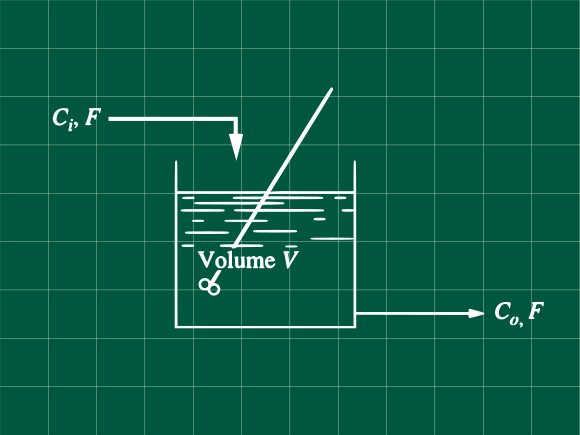
\includegraphics{././images/p5.5-coughanowr/headercontrol.png} Considere
el tanque agitado mostrado en la figura. La reacción que ocurrre es:

\[
A \to B\\
\]

Con una velocidad de reacción igual a:

\[
r=kC_0
\]

Donde

\[
\begin{array}{l}
r \text{ = (mol A)/(volumen)/(tiempo)}\\
k \text{ = constante de velocidad de reacción}\\
C_0(t)\text{ = concentración de A en el reactor en el tiempo t } (mol\space A)/(volumen)\\
V\text{ = volumen de la mezcla en el reactor}\\
F\text{ = caudal de alimentación constante (volumen)/(tiempo)}\\
C_i(t)\text{concentración de A en la entrada (mol A)/(volumen)}
\end{array}
\]

Asumiendo densidad y volumen constante V, derive la función de
tranferencia, relacionando la concentración en el reactor y la
concentración de entrada. Dibuje la respuesta del reactor para un cambio
tipo paso unitario en la concentración de entrada.

\hypertarget{resolviendo-1}{%
\subsection{Resolviendo}\label{resolviendo-1}}

Escribiendo nuestro balance de materia, sabiendo que \(n_o = C_0V\)

\[
C_iF-C_0F-kC_0V=\frac{dn_o}{dt} = \frac{d(C_0V)}{dt}
\]

\[
C_iF-C_0F-kC_0V=V \frac{d(C_0)}{dt} \space\space\space\space\space\textbf{(1)}
\]

Realizando el balance en estado estacionario

\[
C_{is}F-C_{0s}F-kC_{0s}V=0 \space\space\space\space\space\textbf{(2)}
\]

Restado (2) de (1) y tranformando a variables desviación

\[
C_iF-C_{is}F-(C_0F-C_{0s}F)-k(C_0V-C_{0s}V)=V \frac{d(C_0-C_{0s})}{dt}
\]

\[
C'_iF-C'_0F-kC'_0V=V \frac{d(C'_0)}{dt} 
\]

Aplicando la transformada de Laplace y despejando y sabiendo que
\(C'_0(t=0) = 0\)

\[
C'_i(s)F-C'_0(s)F-kC'_0(s)V=V (sC'_0(s)-C'_0(t=0))
\]

\[
C'_i(s)F-C'_0(s)F-kC'_0(s)V=V sC'_0(s)
\]

Obteniendo nuestra función transferencia

\[
\mathbf{\frac{C'_0(s)}{C'_i(s)}=\frac{F}{Vs+F+kV}}
\]

Para poder hacer la gráfica con la variación de la concentración de
entrada, reordenemos nuestra función.

\[
\frac{C'_0(s)}{C'_i(s)}=\frac{F/(F+kV)}{Vs/(F+kV)+1}
\]

Haciendo un cambio de variable

\[
K_p = F/(F+kV)\\
\tau = V/(F+kV)\\
\]

\[
\frac{C'_0(s)}{C'_i(s)}=\frac{K_p}{\tau s+1}
\]

Para un cambio en la concentración de entrada tipo paso unitario Con A
como una constante cualquiera \(C'_i=A/s\).

\[
C'_0(s)=\frac{A}{s}\frac{K_p}{\tau s+1}
\]

Reordenando para realizar la antitransformada

\[
C'_0(s)=\frac{A\cdot K_p+A\cdot K_p \cdot\tau s-A\cdot K_p \cdot\tau s}{s(\tau s+1)}
\]

\[
C'_0(s)=\frac{A\cdot K_p}{s}-\frac{A\cdot K_p \cdot\tau}{\tau s+1}
\]

\[
C'_0(s)=\frac{A\cdot K_p}{s}-\frac{A\cdot K_p}{s+1/\tau}
\]

Antitransformando

\[
C'_0(t) = A\cdot K_p(1-e^{-t/\tau})
\]

Graficando esta respuesta

\begin{figure}

{\centering 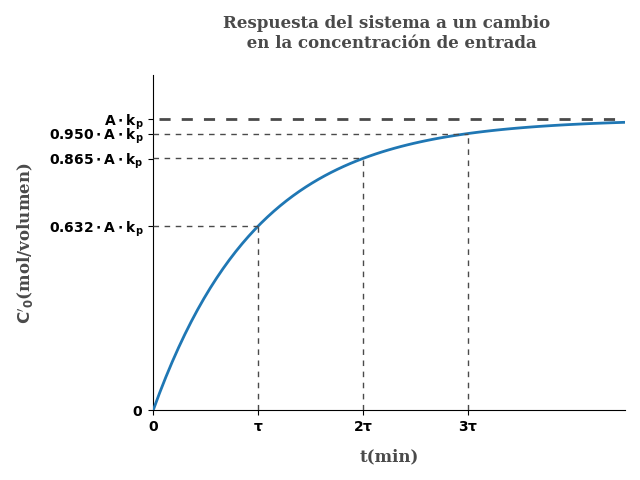
\includegraphics{././images/p5.5-coughanowr/p55r.png}

}

\caption{respuesta del sistema a un cambio en la concentración de
entrada}

\end{figure}

\hypertarget{referencias-4}{%
\section{Referencias}\label{referencias-4}}

\begin{itemize}
\tightlist
\item
  Coughanowr, D. R.; LeBlanc, S. E. (2009). \emph{Process Systems
  Analysis and Control} (3rd edition). McGraw-Hill. ISBN
  978-0-07-339789-4.
\end{itemize}

\hypertarget{termocupla-expuesta-a-un-pulso-rectangular-de-temperatura}{%
\chapter{Termocupla expuesta a un pulso rectangular de
temperatura}\label{termocupla-expuesta-a-un-pulso-rectangular-de-temperatura}}

\begin{figure}

{\centering 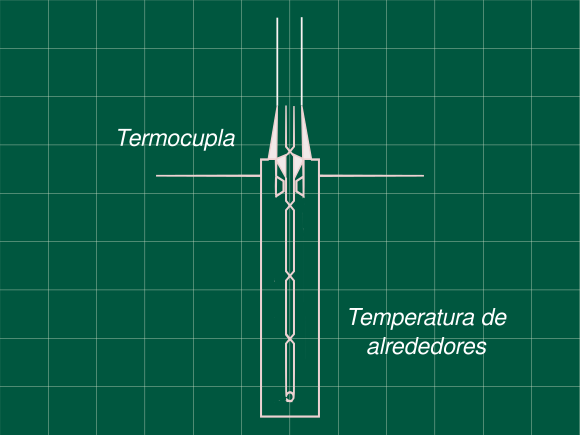
\includegraphics{././images/p5.5-seborg/headercontrol55s.png}

}

\caption{diagrama p5.5}

\end{figure}

Una termocupla tiene las siguientes características cuando es sumergido
en un tanque agitado:

\$\$

\begin{array}{rl}
Masa\ termocupla\ & =\ 1\ g\\
Capacidad\ calorífica\ & =\ 0.25\ cal/(cm^2\ °C)\\
Coeficiente\ de\ transferencia\ de\ calor\  & =\ 20\ cal/(cm^2\ h\ °C)\\
Área\ de\ superficie\ de\ la\ termocupla\ & =\ 3\ cm^2\\

\end{array}

\$\$

Halle la función transferencia de la termocupla que relaciona la
temperatura de la termocupla \(T\) y la de la de los alrededores
\(T_A\).

Si la termocupla esta inicialmente fuera tanque, con una temperatura
ambiente de 23 °C. ¿Cuál será la máxima temperatura alcanzada si es
puesta en el tanque a temperatura de 80 °C, y se la saca después de 20s?

Grafique las la variación de temperatura de la termocupla.

\hypertarget{hallando-la-funciuxf3n-transferencia}{%
\subsection{Hallando la función
transferencia}\label{hallando-la-funciuxf3n-transferencia}}

Escribiendo el balance de energía en estado transitorio y en estado
estacionario.

\[
mC_p\frac{dT}{dt}=UA(T_A-T)
\]

\[
0=UA(T_{As}-T_s)
\]

Restando ambas ecuaciones y pasando a variables desviación

\[
m C_p \frac{d(T-T_s)}{dt}=UA\big[(T_A-T_{As})-(T-T_s)\big]
\]

\[
mC_p\frac{dT'}{dt}=UA(T'_A-T')
\]

Aplicando la transformada de Laplace, sabiendo que para el estado
estacionario T'(t=0)=0

\[
mC_ps\space T(s)=UA(T'_A(s)-T'(s))
\]

Despejando la función tranferencia y haciendo \(\tau = (mC_p)/(UA)\) en
segundos

\[
\frac{T'(s)}{T'_A(s)}=\frac{1}{\tau s+1}
\]

\[
\tau = \frac{1\ g\ \times 0.25\ \frac{cal}{g\ °C}}{20\frac{cal}{cm^2\ h\ °C}\times \frac{1\ h}{360\ s}3\ cm^2}
\] \[
\tau = 15
\]

\[
\mathbf{\frac{T'(s)}{T'_A(s)}=\frac{1}{15 s+1}}\space\space\space\space\textbf{... (1)}
\]

\hypertarget{describiendo-la-perturbaciuxf3n}{%
\subsection{Describiendo la
perturbación}\label{describiendo-la-perturbaciuxf3n}}

\[
T'_A(t)= T_A(t)-T_{As}
\begin{cases}
   0 &\text{si } t < 0 \\
   80-23\ °C &\text{si } 0< t < 20\\
   0 &\text{si } t>20\\
\end{cases}
\]

\[
T'_A(t)=57u(t)-57u(t-20)
\]

Aplicando la antitransformada

\[
T'_A(s)= \frac{57}{s}-57\frac{e^{-20s}}{s}
\]

Reemplanzando en la ecuación (1)

\[
T'(s)=\frac{57}{s(15 s+1)}-\frac{57e^{-20s}}{s(15 s+1)}
\]

Realizando la antitransformada (de tablas). Recuerde que \(e^{-as}\)
crea un desfase en la antitransformada igual a \(t= t-a\)

\[
T´(t)=57(1-e^{-t/15})u(t)-57(1-e^{-t/15})u(t)|_{t=t-20}
\]

\[
T´(t)=57(1-e^{-t/15})u(t)-57(1-e^{-(t-20)/15})u(t-20)
\]

\[
T(t)=T'(t)+T_s
\] \[
T(t)=57(1-e^{-t/15})u(t)-57(1-e^{-(t-20)/15})u(t-20)+23
\] Expresando esta función de manera más entendible

\[
T(t)= 
\begin{cases}
   57(1-e^{-t/15})+23 &\text{si  } 0<t< 20 \\
   57(-e^{-t/15}+e^{-(t-20)/15})+23 &\text{si  } t > 20\\
\end{cases}
\]

Las funciones son monotonicas en ambos rangos, por lo que para el máximo
bastará con analizar el punto anguloso, la temperatura máxima se da un
instante antes de sacar la termocupla del tanque a 80 °C, es decir a los
20 s.

\[
T(t=20)=57(1-e^{-20/15})+23
\]

\[
\mathbf{T_{max}=64.974\ °C}
\]

\hypertarget{gruxe1fica-de-la-funciuxf3n}{%
\subsection{Gráfica de la función}\label{gruxe1fica-de-la-funciuxf3n}}

\begin{figure}

{\centering 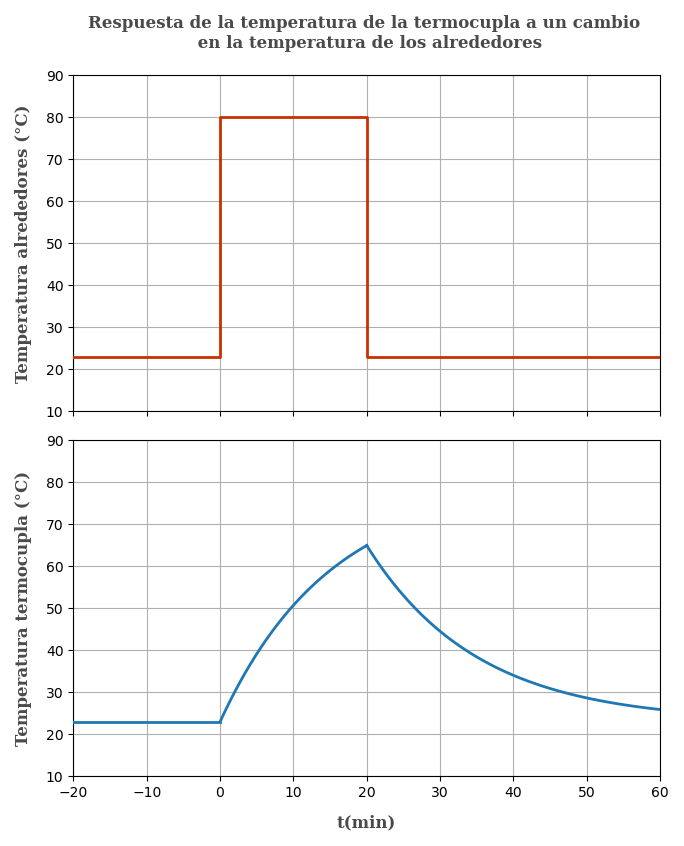
\includegraphics{././images/p5.5-seborg/p55sr.png}

}

\caption{Respuesta temperatura}

\end{figure}

\hypertarget{referencias-5}{%
\section{Referencias}\label{referencias-5}}

\begin{itemize}
\tightlist
\item
  Seborg, D. E.; Edgar, T. F.; Mellichamp, D. A.; Doyle, F. J. (2016).
  \emph{Process Dynamics and Control} (4th edition). John Wiley \& Sons,
  Inc.~ISBN 978-1-119-28591-5.
\end{itemize}

\hypertarget{respuesta-de-un-tanque-a-una-perturbaciuxf3n-tipo-impulso-unitario}{%
\chapter{Respuesta de un tanque a una perturbación tipo impulso
unitario}\label{respuesta-de-un-tanque-a-una-perturbaciuxf3n-tipo-impulso-unitario}}

\begin{figure}

{\centering 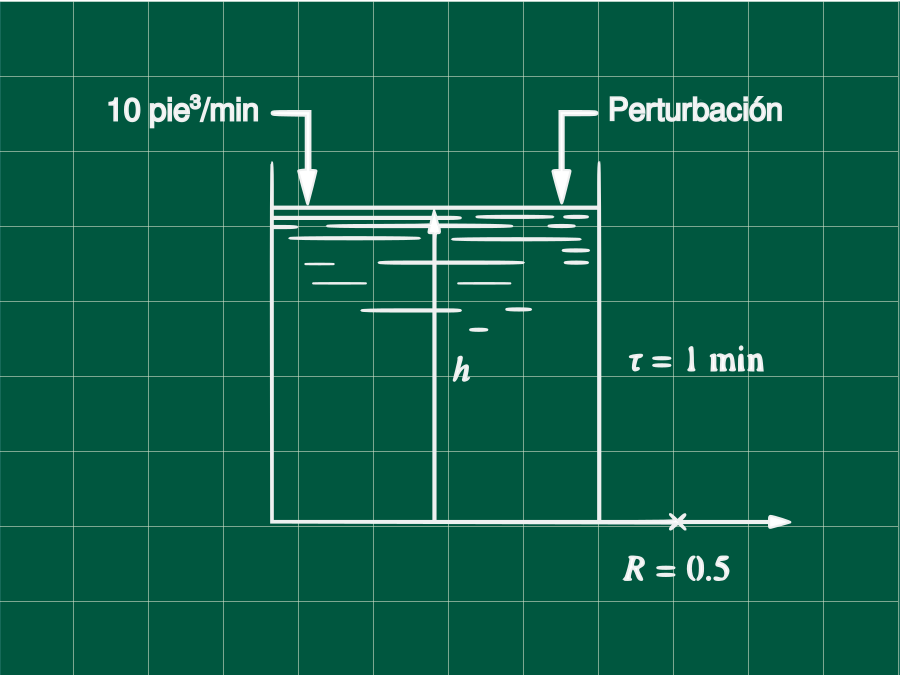
\includegraphics{././images/p5.9-coughanowr/control1.png}

}

\caption{p5.9}

\end{figure}

El nivel del líquido del proceso mostrado en la figura opera en estado
estacionario, entonces una perturbación ocurre. A t = 0,la cantidad de 1
pie³ de agua es añadida al tanque de manera repentina (impulso
unitario); a t = 1min, son añadidos 2 pie³ de agua de manera repentina
también. Dibuje al respuesta del nivel en el tanque (h) vs el tiempo
(t), y determine el nivel en los tiempos t = 0.5, 1.0 y 1.5 minutos. \[
\begin{array}{l}
Datos\\
\tau = 1\text{ min}\\
R = 0.5\\
q_s = 10\space pie³/min
\end{array}
\]

\hypertarget{obtenciuxf3n-de-la-ecuaciuxf3n-en-transferencia}{%
\subsection{Obtención de la ecuación en
transferencia}\label{obtenciuxf3n-de-la-ecuaciuxf3n-en-transferencia}}

Sea \(q\) el caudal, \(h\) el nivel del líquido

Escribiendo las ecuaciones de balance volumétrico \[
q - q_0 = \frac{dV}{dt}
\]

Pero \(q_0 = h/R\) y \(dV = Adh\)

\[
q- \frac{h}{R} = A\frac{dh}{dt} \space\space\space\space (1)
\]

Escribiendo el balance en estado estacionario

\[
q_s- \frac{h_s}{R} = 0 \space\space\space\space (2)
\]

Restando (1) con (2) para obtener las variables desviación y recordando
que \(dh=d(h-h_s)\), por ser \(h_s\) constante.

\[
q-q_s-\frac{h-h_s}{R}=A\frac{d(h-h_s)}{dt}
\]

\[
Q - \frac{H}{R} = A\frac{dH}{dt}
\]

Aplicando la tranformada de Laplacey sabiendo que
\(H(t=0)= h-h_s=h_s-h_s=0\)

\[
Q(s) - \frac{H(s)}{R} = A\left[sH(s)-H(t=0)\right]\\
\\
Q(s) - \frac{H(s)}{R} = AsH(s)
\]

Despejando y sabiendo que \(\tau=AR\)

\$\$

\frac{H(s)}{Q(s)}=\frac{R}{ARs+1} \textbackslash{} \[
\] \frac{H(s)}{Q(s)}=\frac{R}{\tau s+1} \textbackslash{}

\$\$

Reemplazando los valores \(\tau = 1\) y \(R=0.5\)

\[
\frac{H(s)}{Q(s)}=\frac{0.5}{s+1} \space\space\space\space (3)\\
\]

\hypertarget{descripciuxf3n-de-la-perturbaciuxf3n-1}{%
\subsection{Descripción de la
perturbación}\label{descripciuxf3n-de-la-perturbaciuxf3n-1}}

La perturbación sólo va a afectar el caudal de ingreso, esta puede ser
representado por la variable desviación \(Q(t)\). Para diferenciar el
impulso unitario se pondrá el simbolo de \(\infty\) al lado del valor de
la perturbación.

\[
Q(t)=
\begin{cases}
   0 &\text{si } t < 0 \\
   1 \space\ pie³/min\space \space\space(\infty) &\text{si } t=0\\
   0 \space\  &\text{si } t>0\\
   2 \space\ pie³/min\space\space\space (\infty) &\text{si } t=1 min\\
\end{cases}
\]

Expresando la misma función con impulsos unitarios y aplicando la
transformada de Laplace

\[
\begin{array}{l}
Q(t) = 1 \cdot \delta (t) + 2 \cdot \delta (t-1) \space\space\space\space //L\{\space\}\\
Q(s) = 1 + 2\cdot e^{-s}\cdot L\{ \delta (t) \}\\
Q(s) = 1 + 2 \cdot e^{-s}
\end{array}
\]

Reemplazando la expresión anterior en la ecuación (3)

\[
\begin{array}{l}
H(s)= Q(s)\cdot \frac{0.5}{s+1} \\
\\
H(s) = \left(1+2e^{-s}\right)\frac{0.5}{s+1}\\
\end{array}
\]

Despejando y aplicando la antitransformada \(L^{-1}\{\space\}\) Recuerde
que la expresión \(e^{-as}\) crea un desfase de tiempo en la
antitranformada igual a \(t-a\), también
\(L^{-1}\{\frac{1}{s+k}\}= e^{-kt}\)

\[
H(s) = \frac{0.5}{s+1}+\frac{e^{-s}}{s+1}\\
\]

\[
\begin{array}{l}
H(t) = 0.5\cdot e^{-t} \cdot u(t)+ e^{-t}\cdot u(t) |_{t=t-1}\\
\\
H(t) = 0.5\cdot e^{-t}\cdot u(t) + e^{-(t-1)} \cdot u(t-1)
\end{array}
\]

\emph{Notese que normalmente se omite el término \(u(t)\) en la
antitransformada, pero en este caso es necesario ponerlo para aclarar
los dominios}

Escribiendo nuestra ecuación de manera más entendible

\[
H(t)=
\begin{cases}
   0.5\cdot e^{-t} &\text{si }\space 0 < t < 1\\
   0.5\cdot e^{-t} + e^{-(t-1)} &\text{si } \space t>1\\
\end{cases} \space\space\space\space\space \textbf {(4)}
\]

Con las funciones ya determinadas podemos graficarlas.

\begin{figure}

{\centering 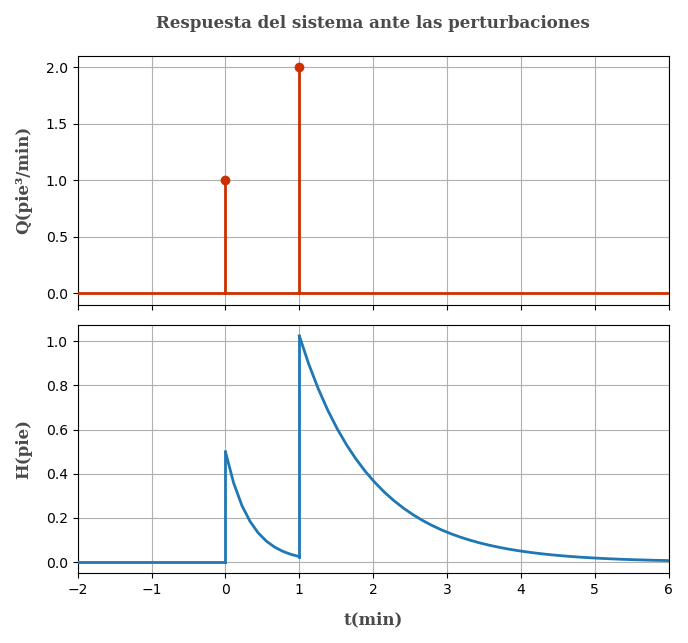
\includegraphics{././images/p5.9-coughanowr/p5.9r.png}

}

\caption{p5.9 respuesta del sistema}

\end{figure}

Del enunciado nos piden calcular las el valor de \(h(t=0.5)\),
\(h(t=1)\) y \(h(t=1.5)\)

Recuerde que \(H = h-h_s\) por que lo que \(h=H+h_s\)

Determinado \(h_s\) de la ecuación del estado estacionario

\[
q_s- \frac{h_s}{R} = 0\\
\\
h_s = q_s \cdot R = 10\cdot 0.5 = 5 pie
\]

Usando la ecuación (4) para hallar lo solicitado

\[
\begin{array}{l}
h(t=0.5) = H(t=0.5)+5\\
\\
\mathbf{h(t=0.5) = 0.5\cdot e^{-0.5} + 5 = 5.3033\text{ pie}}
\end{array}
\]

Para cuando t = 1 min nuestra función matemática no esta definida (los
puntos en la gŕafica son punteagudos y hay una pendiente infinita) pero
si la tenemos definida antes y despues de la perturbación, teniendo eso
en cuenta y sabiendo que nuestro modelo es una aproximación del
fenómeno, indicamos que la altura inmediatamente antes de la
perturbación a t = 1 min es:

\[
h(t=1)= 0.5\cdot e^{-1} + 5\\
\]

\[
\mathbf{h(t=1)=5.1839\text{ pie}}
\]

E inmediatamente después de la perturbación a 1 minuto

\[
h(t=1)= 0.5\cdot e^{-(1-1)}+e^{-1} + 5\\
\]

\[
\mathbf{h(t=1) = 6.1839\text{ pie}}
\]

A t = 1.5 min

\[
h(t=1.5)= 0.5\cdot e^{-1.5} + e^{-(1.5-1)} + 5\\
\]

\[
\mathbf{h(t=1.5)= 5.7181\text{ pie}}\\
\]

Para completar el ejercicio, grafiquemos el nivel del líquido en el
tiempo (h vs t)

La grafíca es similar a la gráfica de H(t) vs t, con la diferencia de
que esta desplazado en el eje de las ordenadas.

\begin{figure}

{\centering 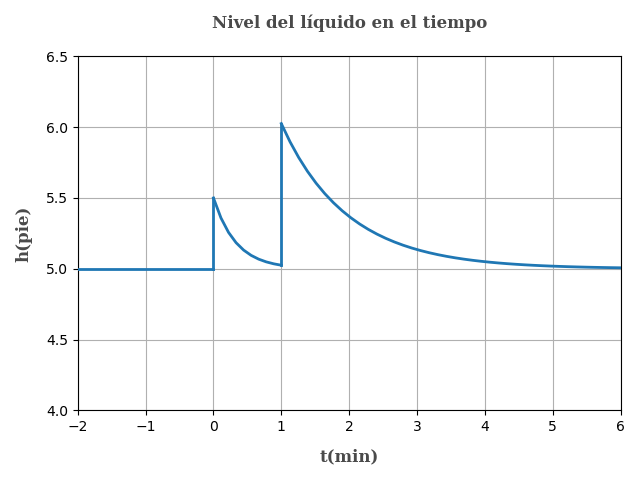
\includegraphics{././images/p5.9-coughanowr/hvst.png}

}

\caption{h vs t}

\end{figure}

\hypertarget{referencias-6}{%
\section{Referencias}\label{referencias-6}}

\begin{itemize}
\tightlist
\item
  Coughanowr, D. R.; LeBlanc, S. E. (2009). \emph{Process Systems
  Analysis and Control} (3rd edition). McGraw-Hill. ISBN
  978-0-07-339789-4.
\end{itemize}

\hypertarget{dos-tanques-uno-con-una-vuxe1lvula-y-el-otro-con-una-bomba}{%
\chapter{Dos tanques uno con una válvula y el otro con una
bomba}\label{dos-tanques-uno-con-una-vuxe1lvula-y-el-otro-con-una-bomba}}

\begin{figure}

{\centering 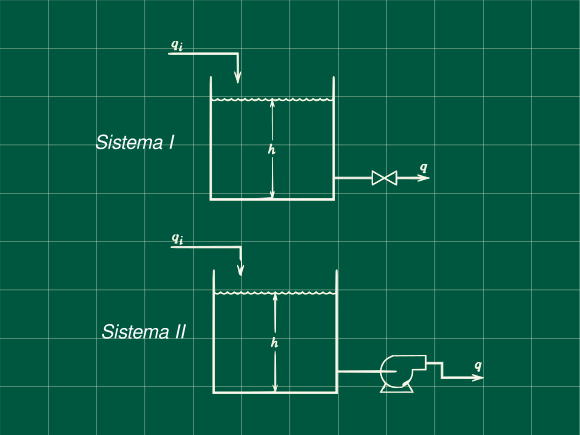
\includegraphics{././images/p5.9-seborg/headercontrol59s.png}

}

\caption{diagrama p5.9}

\end{figure}

Dos tanques mostrados en la figura, cada uno tiene un diámetro de 4 pie,
Para el primer sistemas la válvula tiene una resistencia linear con la
ecuación \(q = 8.33\  h\) con q en (gal/min) y h en (pie). Para el
segundo sistema, la variación en el nivel del líquido no afecta el
caudal de salida \(q\) . Suponga que cada sistema esta inicialmente en
estado estacionario con \(h_s = 6\ pie\) y \(q_s = 50\ gal/min\). A
\(t=0\) el caudal de entrada se incrementa de 50 a 70 gal/min.

Determine para cada sistema

\begin{enumerate}
\def\labelenumi{\alph{enumi})}
\item
  La función transferencia \(H(s)/Q(s)\)
\item
  La función h(t)
\item
  Los nuevos estados estacionario
\item
  Si cada tanque tiene 8 pie de altura, ¿cuál tanque rebalsa primero y
  cuando?
\item
  Verifique los resultado en d) graficando lo resultados
\end{enumerate}

\hypertarget{datos}{%
\subsection{Datos}\label{datos}}

\[
\begin{array}{rl}
d = &4 pie\\
h_s= &6 pie\\
q_{is}=&50\ gal/min\\
q_i=&70\ gal/min\\
h_s=&8\ pie\\
q=&8.33\ h\ gal/min
\end{array}
\]

Estandarizamos los datos anteriores (es decir convertimos a unidades
compatibles) y obtenemos el área de los tanques. (7.48 gal = 1 pie³) \[
\begin{array}{l}
A\ = \frac{\pi d^2}{4}\ =\ 12.5665\ pie^2\\
\\
q_{is}\ =50/7.48\ =\ 6.6845\ pie^3/min\\
\\
q_i\ =\ 9.3583\ pie^3/min\\
\\
q\ =\ 8.33\frac{gal}{min\cdot pie}\ h \frac{1\ pie^3}{7.48\ gal} = 1.1136\ h\\
\end{array}
\]

Para simplificar las operaciones hagamos \(q=kh\) con \(k=1.1136\)

\hypertarget{derivaciuxf3n-de-la-ecuaciuxf3n-tranferencia-para-el-primer-tanque}{%
\subsection{Derivación de la ecuación tranferencia para el primer
tanque}\label{derivaciuxf3n-de-la-ecuaciuxf3n-tranferencia-para-el-primer-tanque}}

Escribiendo las ecuaciones de balance de materia (asumiendo densidad
constante) en estado transitorio y en estado estacionario:

\[
A\frac{dh}{dt}= q_i-kh
\]

\[
0=q_{is}-kh_s
\]

Restando ambas ecuaciones y pasando a variables desviación

\[
A\frac{dH}{dt}=Q_i-kH
\]

Aplicando la transformada de Laplace

\[
AsH(s)=Q_i(s)-kH(s)
\]

\[
\frac{H(s)}{Q(s)}=\frac{1/K}{As/K+1}
\]

Reemplazando valores conocidos

\[
\mathbf{\frac{H(s)}{Q(s)}=\frac{0.8980}{12.2845s+1}}\space\space\space\space\textbf{... (1)}
\]

\hypertarget{obteniendo-la-funciuxf3n-transferencia-para-el-segundo-sistema}{%
\subsection{Obteniendo la función transferencia para el segundo
sistema}\label{obteniendo-la-funciuxf3n-transferencia-para-el-segundo-sistema}}

Planteando los balances en estado transitorio y estacionario con \(q_b\)
para el caudal de la bomba

\[
A\frac{dh}{dt}=q_i-q_b
\]

\[
0=q_{is}-q_b
\]

Restando ambas ecuaciones y conviertiendo a variables desviación

\[
A\frac{d(h-h_s)}{dt}=q_i-q_{is}
\] \[
A\frac{dH}{dt}=Q_i
\]

Aplicando la transformada de Laplace y despejando la función
tranferencia

\[
AsH(s)=Q_i(s)
\]

\[
\frac{H(s)}{Q_i(s)}=\frac{1}{As}
\]

Reemplazando datos conocidos

\[
\mathbf{\frac{H(s)}{Q_i(s)}=\frac{1}{12.5664s}} \space\space\space\space\textbf{... (2)}
\]

\hypertarget{respuesta-de-los-sistema-a-la-perturbaciuxf3n}{%
\subsection{Respuesta de los sistema a la
perturbación}\label{respuesta-de-los-sistema-a-la-perturbaciuxf3n}}

Decripción de la perturbación

\[
Q(t)= q(t)-q_s
\begin{cases}
   q_s-q_s&\text{si } t < 0 \\
   q_i-q_s &\text{si } t > 0\\
\end{cases}
\]

\[
Q(t)= q(t)-6.6845
\begin{cases}
   0&\text{si } t < 0 \\
   9.3583-6.6845=2.6738 &\text{si } t > 0\\
\end{cases}
\]

\[
\begin{array}{lcr}
Q(t)=2.6738u(t)&\rightarrow & Q(s)=\frac{2.6738}{s}\\
\end{array}
\]

\[
\mathbf{Q(s)=\frac{2.6738}{s}}
\]

Reemplazando en la ecuación (1) \(Q(s)=\frac{2.6738}{s}\)

\[
H(s)=\frac{2.6738\times 0.8980}{s(12.2845s+1)}
\]

Separando en fracciones parciales y aplicando la antitransformada (Puede
reemplazar de tablas directamente)

\[
H(s)=2.4011\left(\frac{1}{s}-\frac{1}{s+1/12.2845}\right)
\]

\[
H(t)=2.4011(1-e^{-t/12.2845})
\]

Recordando que \(H(t)=h(t)-h_s\) con \(h_s=6\ pie\)

\[
h(t)=2.4011(1-e^{-t/12.2845})+6
\]

Calculanado para que tiempo se llegará a una altura de h=8

\[
8=2.4011(1-e^{-t/12.2845})+6
\]

\[
t=-12.2845ln\left(1-\frac{2}{2.4011}\right)
\]

\[
\mathbf{t_I=21.98\ min}
\]

Calculando el nuevo estado estacionario para el primer sistema

\[
h(t\to\infty)=\lim_{t\to\infty}2.4011(1-e^{-t/12.2845})+6 
\]

\[
\mathbf{h_{sI}= 8.4011\ pie}
\]

Para el sistema 2 reemplazando (2) \(Q(s)=\frac{2.6738}{s}\)

\[
H(s)=\frac{2.6738}{s(12.5664s)}
\]

Realizando la antitranformada y despejando para \(h(t)\)

\[
H(t)=0.2128\cdot t
\]

\[
h(t)=0.2128t+6
\]

El tiempo para el cual \(h = 8\)

\[
8=0.2128t+6
\]

\[
\mathbf{t_{II}=9.40\ min}
\]

Calculando el nuevo estado estacionario para el sistema II

\[
h(t\to\infty)=\lim_{t\to\inf}0.2128t+6
\]

\[
\mathbf{h_{sII}=\infty}
\]

Es decir el sistema 2 no tiene un nuevo estado estacionario y tiende al
infinito.

Siendo que \(t_{II}<t_I\) determinamos que el \textbf{sistema II rebalsa
primero}

Graficando ambos sistemas

\begin{figure}

{\centering 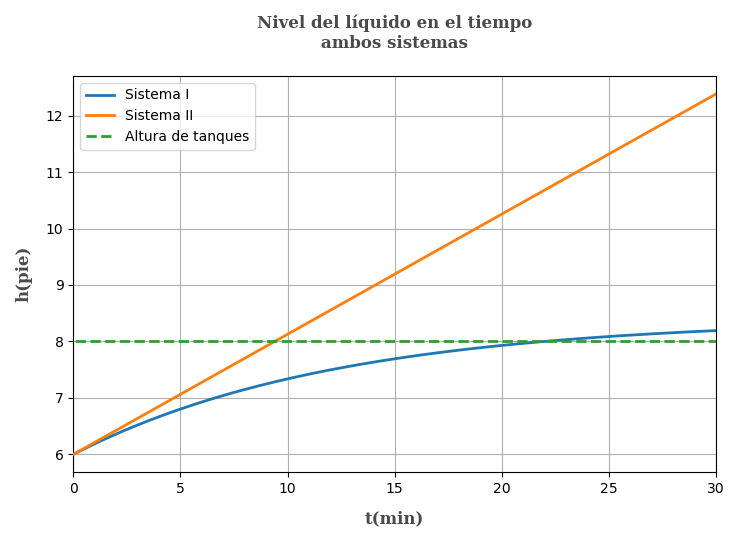
\includegraphics{././images/p5.9-seborg/p59sr.png}

}

\caption{Altura de líquidos de ambos sistemas}

\end{figure}

\hypertarget{referencias-7}{%
\section{Referencias}\label{referencias-7}}

\begin{itemize}
\tightlist
\item
  Seborg, D. E.; Edgar, T. F.; Mellichamp, D. A.; Doyle, F. J. (2016).
  \emph{Process Dynamics and Control} (4th edition). John Wiley \& Sons,
  Inc.~ISBN 978-1-119-28591-5.
\end{itemize}

\hypertarget{reactor-quuxedmico-con-una-velocidad-de-reacciuxf3n-cuadruxe1tica}{%
\chapter{Reactor químico con una velocidad de reacción
cuadrática}\label{reactor-quuxedmico-con-una-velocidad-de-reacciuxf3n-cuadruxe1tica}}

\begin{figure}

{\centering 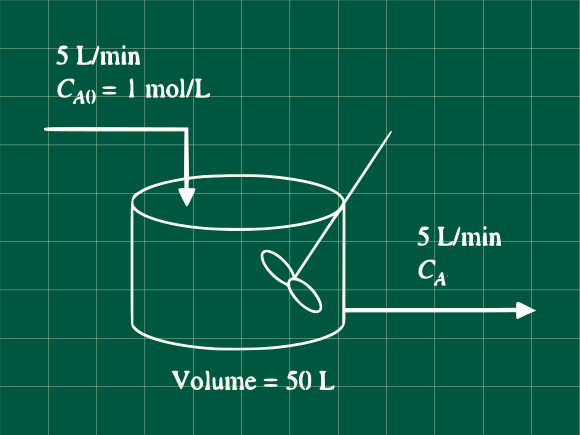
\includegraphics{././images/p5.16-coughanowr/headercontrol516.png}

}

\caption{gráfica problema 5.16}

\end{figure}

Para el reactor de mezcla completa mostrada en la figura, determine la
función de transferencia que relaciona la concentración de salida con la
concentración de la alimentación. Si cambiamos la concentración de
entrada de 1 a 2 mol/L, ¿Cuál es la nueva concentración de salida? y
¿Cuál es la concentración en el nuevo estado estacionario?

Nuestros datos

\[
k = \frac{2\cdot L}{mol\cdot min}
\]

Reacción

\[
2A\Rightarrow B\\
\]

\[
-r_A=kC_A^2
\]

\hypertarget{resolviendo-2}{%
\subsection{Resolviendo}\label{resolviendo-2}}

Linealicemos el término cuadrático antes. Usando la serie de Taylor
truncada a primer orden

\[
f(x)=f(x_s)+\frac{df}{dx}\bigg |_{x=x_s} (x-x_s)
\]

Siendo nuestra función a linealizar \(f(C_{A})=C_A^2\)

\[
C_A^2=C_{As}^2+2\cdot C_{As}(C_A-C_{Aas})
\]

\[
C_A^2-C_{As}^2=2\cdot C_{As}(C_A-C_{Aas})\space\space\space\space\space\textbf{... (1)}
\]

Escribiendo nuestro balance de materia, sabiendo que \(n_o = C_0V\)

\[
C_{A0}F-C_AF-kC_A^2V=\frac{dn_o}{dt} = \frac{d(C_AV)}{dt}
\]

\[
C_{A0}F-C_AF-kC_A^2V=V \frac{d(C_A)}{dt} \space\space\space\space\space\textbf{... (2)}
\]

Realizando el balance en estado estacionario

\[
C_{A0s}F-C_{As}F-kC_{As}^2V=0 \space\space\space\space\space\textbf{... (3)}
\]

Restado (3) de (2). Recuerde que \(d(C_A)=d(C_A-C_{As})\)

\[
(C_{A0}-C_{A0s})F-(C_A-C_{As})F-(C_A^2-C_{As}^2)kV=V \frac{d(C_A-C_{As})}{dt}
\]

Transformando a variables desviación y reemplazando la ecuación (1)

\[
C'_{A0}F-C'_AF-\big[2C_{As}(C_A-C_{As})\big]kV=V \frac{d(C'_A)}{dt}
\]

\[
C'_{A0}F-C'_AF-2C_{As}(C'_A)kV=V \frac{d(C'_A)}{dt}
\]

Aplicando la transformada de Laplace y despejando y sabiendo que
\(C'_A(t=0) = 0\)

\[
C'_{A0}(s)F-C'_A(s)F-2C_{As}C'_A(s)kV=V (sC'_A(s)-C'_A(t=0))
\]

\[
FC'_{A0}(s)-FC'_A(s)-2C_{As}kVC'_A(s)=V sC'_A(s)\space\space\space\space\space\textbf{... (4)}
\]

Para simplificar el manejo de la ecuación (4) necesitamos reemplazar
datos, pero nos falta conocer un dato \(C_{As}\), para hallar utilizamos
la ecuación (3), conociendo que: \(k = 2;\space\space\)
\(C_{A0s} = 1;\space\space\) \(V=50\space\space\) y \(\space F= 5\)

\[
5\times 1-5\times C_{As}-2\times 50\times C_{As}^2=0
\]

\[
1-C_{As}-20\times C_{As}^2=0
\] Usando la formula cuadrática para resolver \(C_{As}\) y sólo tomando
en cuenta el valor positivo

\[
C_{As}=\frac{-1±\sqrt{1+4\times 20}}{2\times 20}
\] \[
C_{As}=\frac{-1+9}{40}
\] \[
C_{As}=0.2
\] Reemplazando en la ecuación (4) \[
5C'_{A0}(s)-5C'_A(s)-2\times 0.2\times 2\times 50\times C'_A(s)=50\times sC'_A(s)
\]

\[
C'_{A0}(s)-9C'_A(s)=10 sC'_A(s)
\]

\[
\mathbf{\frac{C'_{A}(s)}{C'_{A0}(s)}=\frac{1}{10s+9}}\space\space\space\space\space\textbf{... (5)}
\]

Describiendo la perturbación

\[
C'_{A0}(t)=C_{A0}-C_{A0s}=
\begin{cases}
   1 - 1 &\text{si } t < 0 \\
   2 - 1 \space\ mol/L &\text{si } t>0\\
\end{cases}
\]

\[
C'_{A0}(t)=
\begin{cases}
   0 &\text{si } t < 0 \\
   1 \space\ mol/L &\text{si } t>0\\
\end{cases}
\]

\[
C'_{A0}(t)= 1\space u(t)
\]

Entonces su transforma da de Laplace es

\[
C'_{A0}(s)= \frac{1}{s}
\]

Reemplazando en la ecuación (5)

\[
C'_{A}(s)=C'_{A0}\frac{1}{10s+9}
\]

\[
C'_{A}(s)=\frac{1}{s(10s+9)}
\]

Reordenando para obtener la antitransformada (Recuerde que tambien puede
obtener la antitransformada directamente de tablas)

\[
C'_{A}(s)=\frac{9}{9s(10s+9)}=\frac{9+10s-10s}{9s(10s+9)}
\]

\[
C'_{A}(s)=\frac{9+10s}{9s(10s+9)}-\frac{10s}{9s(10s+9)}
\]

\[
C'_{A}(s)=\frac{1}{9s}-\frac{10}{9(10s+9)}
\]

\[
C'_{A}(s)=\frac{1}{9s}-\frac{1}{9(s+9/10)}
\]

Antitransformando

\[
C'_A(t) = \frac{1}{9}-\frac{1}{9}e^{-9t/10}
\]

Hallando la concentración cuando t = 1 min

\$\$ C\_A(t=1) = C'\emph{A(t=1)+C}\{As\}

\$\$

\[
C_A(t=1)=\frac{1}{9}(1-e^{-9/10})+0.2
\]

\[
\mathbf{C_A(t=1\textbf{ min})=0.2659\textbf{ mol/L}}
\] Para hallar la nueva concentración en el estado estacionario hacemos
que el tiempo tienda a infinito (\(t\to\infty\))

\[
C_A(t\to\infty)=\lim_{t\to\infty}\left(\frac{1}{9}(1-e^{-9t/10})+0.2\right)
\]

\[
\mathbf{C_A(t\to\infty)=\textbf{ 0.3111 mol/L}}
\]

\hypertarget{referencias-8}{%
\section{Referencias}\label{referencias-8}}

\begin{itemize}
\tightlist
\item
  Coughanowr, D. R.; LeBlanc, S. E. (2009). \emph{Process Systems
  Analysis and Control} (3rd edition). McGraw-Hill. ISBN
  978-0-07-339789-4.
\end{itemize}

\hypertarget{un-cono-por-tanque-con-una-vuxe1lvula.}{%
\chapter{Un Cono por tanque con una
válvula.}\label{un-cono-por-tanque-con-una-vuxe1lvula.}}

\begin{figure}

{\centering 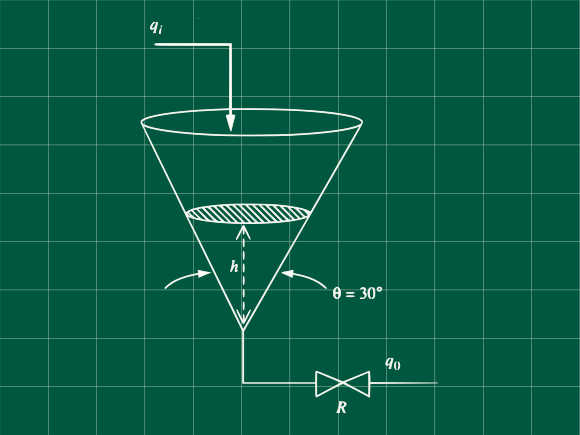
\includegraphics{././images/p5.18-coughanowr/headercontrol518.png}

}

\caption{gráfica problema 5.18}

\end{figure}

Encuentre la función transferencia que relaciona la altura del embudo
tanque y los cambios en el caudal de entrada.

Asumiendo densidad constante, realizamos nuestro balance de materia

\[
q_i-q_o=\frac{dV}{dt}\space\space\space\space\textbf{... }\mathbf{(\alpha)}
\]

Observamos que nuestro volumen es dependiente de la altura de manera no
lineal. Nuestro radio y volumen estan en función de la altura

\[
r = h\cdot tan(15°)
\]

\[
V = \frac{\pi r^2 h}{3}
\]

Poniendo el volumen en función de h, y haciendo \(k_1=\pi tan^2(15°)/3\)
\[
V = \frac{\pi tan^2(15°)}{3}h^3
\]

\[
V = k_1h^3
\]

Linealizando usando la serie de Taylor truncada a primer orden,
alrededor del estado estacionario

\[
f(x)=f(x_s)+\frac{df}{dx}\bigg |_{x=x_s} (x-x_s)
\]

Siendo nuestra función a linealizar \(f(h)=V=k_1h^3\), recuerde que
\(f(h_s)=V_s=k_1h_s^3\)

\[
V=k_1h_s^3+3k_1h_s^2(h-h_s)
\]

\[
V=V_s+3k_1h_s^2(h-h_s)
\]

\[
V-V_s=3k_1h_s^2(h-h_s)
\]

Diferenciando la ecuación convenientemente

\[
d(V-V_s)=3k_1h_s^2\cdot d(h-h_s)\space\space\space\space\textbf{... }\mathbf{(\beta)}
\]

Trabajando en la ecuación \(\alpha\), Asumiendo linealidad de la válvula
entonces reemplazando \(q_o=h/R\)

\[
q_i-\frac{h}{R}=\frac{dV}{dt}\space\space\space\space\textbf{... }\mathbf{(\gamma)}
\]

Reescribiendo la ecuación en estado estacionario

\[
q_{is}-\frac{h_s}{R}=0\space\space\space\space\textbf{... }\mathbf{(\theta)}
\]

Restando \(\theta\) de \(\gamma\) y sabiendo que \(dV=d(V-V_s)\) por ser
\(V_s\) constante.

\[
q_i-q_{is}-\frac{h-h_s}{R}=\frac{d(V-V_s)}{dt}
\]

Reemplazando la ecuación \(\beta\)

\[
q_i-q_{is}-\frac{h-h_s}{R}=3k_1h_s^2\frac{d(h-h_s)}{dt}
\]

Cambiando a variables desviación

\[
Q_i-\frac{H}{R}=3k_1h_s^2\frac{d(H)}{dt}
\]

Aplicando la transformada de Laplace (\(H(t=0) = h_s-h_s = 0\))

\[
Q_i(s)-\frac{H(s)}{R}=3k_1h_s^2(sH(s)-H(t=0))
\]

\[
Q_i(s)-\frac{H(s)}{R}=3k_1h_s^2sH(s)
\]

\[
\frac{H(s)}{Q_i(s)}=\frac{R}{3k_1h_s^2R\cdot s+1}
\]

Reemplazando adecuadamente y sabiendo que \(k_1=\pi \cdot tan^2(15°)/3\)

\[
\frac{H(s)}{Q_i(s)}=\frac{K_p}{\tau s+1}
\]

Con \(\tau =\pi \cdot tan^2(15°)\cdot h_s^2\cdot R\space\space;\)
\(\space\space K_p = R\)

\hypertarget{referencias-9}{%
\section{Referencias}\label{referencias-9}}

\begin{itemize}
\tightlist
\item
  Coughanowr, D. R.; LeBlanc, S. E. (2009). \emph{Process Systems
  Analysis and Control} (3rd edition). McGraw-Hill. ISBN
  978-0-07-339789-4.
\end{itemize}

\hypertarget{una-reacciuxf3n-exotuxe9rmica-un-reactor-con-cambio-de-temperatura}{%
\chapter{Una reacción exotérmica, un reactor con cambio de
temperatura}\label{una-reacciuxf3n-exotuxe9rmica-un-reactor-con-cambio-de-temperatura}}

\begin{figure}

{\centering 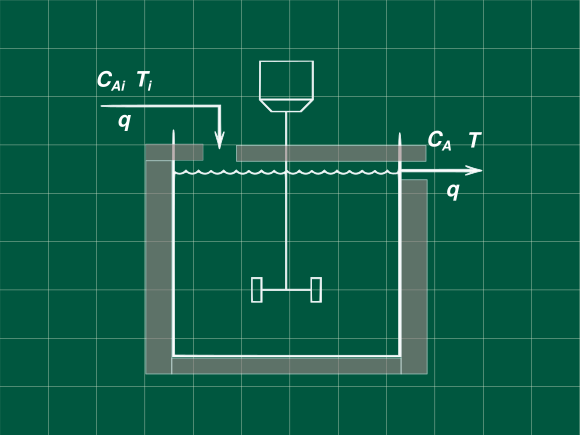
\includegraphics{././images/p5.21-seborg/headercontrol521.png}

}

\caption{diagrama p5.21}

\end{figure}

Una reacción exotérmica toma lugar en un tanque agitado adiabático, La
reacción líquida ocurre a volumen constante V = 100 gal, La reacción
puede ser considerada de primer orden e irreversible dada por la
ecuación \[
k = k_0e^{-E_R/T}
\] Con \(k_0=2.4\times 10^{15}\) y \(E_R = 20\space000\). Donde T esta
en °R, usando los datos proporcionados abajo determine la función
transferencia que relaciona la temperatura de salida T, y la
concentración de entrada CAi, describa lo que se asume para resolverlo.
Simplifique la función transferencia haciendo una aproximación a primer
orden, muestre que es válida con una perturbación tipo escalón
unitario(heaviside) y compare las respuestas con la respuesta original y
la respuesta de función de transferencia no simplificada.

Condiciones de estado estacionario

\[
\begin{array}{ll}
T_s = 150 \space °F & C_{Ais}=0.8\space lb\space mol/pie^3\\
q=20\space gal/min & \\
\end{array}
\]

Propiedades físicas de la mezcla

\[
\begin{array}{ll}
C_p=0.8\text{ BTU/(lb °F)}& \rho=52\text{ lb/pie³}\\
-\Delta H_R = 500\text{ kJ/(lb mol)}\\
\end{array}
\]

Reescribiendo nuestros datos, pero estandarizando unidades. Sabiendo
que: \[
\begin{array}{cc}
T[°R]= T[°F]+459.67 &1\text{ pie³ } = 7.48\text{ gal}\\
1\text{ BTU } = 1.055\text{ kJ}\\
\end{array}
\]

\[
T_s = 609.67 \text{ °R}\\
-\Delta H_R = 473.9336 \text{ BTU/(lb mol)}\\
q = 2.6738 \text{ pie³/min}\\
V = 13.3690\text{ pie³}
\]

Realizando el balance de materia para los moles de A.

\[
V\frac{dC_A}{dt}=q(C_{Ai}-C_A)-Vk(T)C_A \space\space\space\space\textbf{ .... (1)}
\]

Realizando el balance en estado estacionario

\[
0=q(C_{Ais}-C_{As})-Vk(T_s)C_{As}\space\space\space\space\textbf{ .... (2)}
\]

Restado (1) y (2) y adecuando la ecuación para cambiar a variables
desviación

\[
V\frac{d(C_A-C_{As})}{dt}=q\left[(C_{Ai}-C_{Ais})-(C_A-C_{As})\right]-V\left[k(T)C_A-k(T_s)C_{As}\right]
\]

Conviertiendo a variables desviación

\[
V\frac{dC'_A}{dt}=q(C'_{Ai}-C'_A)-V(k(T)C_A-k(T_s)C_{As}) \space\space\space\space\textbf{...(3)}
\]

Linealizando la expresión \(k = k_0e^{E_R/T}\) usando la aproximaciones
en series de taylor al rededor del el punto del estado estacionario.

\[
f(x,y)=f(x_s,y_s)+\frac{df}{dx}\bigg|_{x=x_s}(x-x_s)+\frac{df}{dy}\bigg|_{y=y_s}(y-y_s)
\]

Reemplazando con \(f(T,C_A)=k(T)\cdot C_A\) con \(k(T) = k_0e^{-E_R/T}\)
y \(T\), \(C_A\) como variables independientes

\[
\frac{df}{dT}\bigg|_{T=T_s, C_A=C_{As}}= \frac{k_0E_R}{T_s^2}e^{-E_R/T_s}C_{As}
\]

\[
\frac{df}{dC_{A}}\bigg|_{T=T_s, C_A=C_{As}}= k_0e^{-E_R/T_s}
\\
\]

\[
\\
k(T)C_A = k(T_s)C_{As}+\frac{k_0E_R}{T_s^2}e^{-E_R/T_s}C_{As}(T-T_s)+ k_0e^{-E_R/T_s}(C_A-C_{As})
\]

En variables desviación es:

\[
k(T)C_A - k(T_s)C_{As}=\frac{k_0E_R}{T_s^2}e^{-E_R/T_s}C_{As}T'+ k_0e^{-E_R/T_s}C'_A\textbf{ ... (4)}
\]

Para una ecuación muy extensa es mejor reemplazar cuidadosamente los
datos, pero antes debemos hallar el valor de \(C_{As}\).

Despejando de la ecuación (2) del balance en estado estacionario.

\[
0=q(C_{Ais}-C_{As})-Vk(T_s)C_{As}
\]

\[
0=q(C_{Ais}-C_{As})-Vk_0e^{E_R/T_s}C_{As}
\]

\[
0=2.6738(0.8-C_{As})-13.3690\times 2.4\times 10^{15} e^{-20000/609.67}C_{As}
\]

Despejando

\[
C_{As}=0.0116\text{ lb mol/ pie³}
\]

Ahora reemplazando todos los datos conocidos en la ecuación (4)

\[
\begin{array}{l}
k(T)C_A - k(T_s)C_{As} = \\ \\ \frac{2.4\times 10^{15} 20000}{609.67^2}e^{-20000/609.67}\times 0.00116T'+ 2.4\times 10 ^{15}e^{-20000/609.67}C'_A
\end{array}
\]

\[
k(T)C_A - k(T_s)C_{As} = 0.008485T'+12.2025C'_A \space\space\textbf{ ... (5)}
\]

Reemplazando en la ecuación (3) y reemplazando datos conocidos

\[
V\frac{dC'_A}{dt}=q(C'_{Ai}-C'_A)-V(k(T)C_A-k(T_s)C_{As})
\]

\[
V\frac{dC'_A}{dt}=q(C'_{Ai}-C'_A)-V(0.008485T'+12.2025C'_A)
\]

\[
13.369\frac{dC'_A}{dt}=2.6738(C'_{Ai}-C'_A)-13.369(0.008485T'+12.2025C'_A)
\]

\[
13.3690\frac{dC'_{A}}{dt}=2.6738(C'_{Ai}-C'_A)-0.11343 T'-163.1352C'_A
\]

Aplicando la transformada de Laplace y ordenando

\[
13.369sC'_A(s)=2.6738C'_{Ai}(s)-0.11343T'(s)-165.809C'_A(s)
\]

\[
C'_A(s) = \frac{2.6738C'_{Ai}(s)-0.11343T'(s)}{13.369s+165.809}\space\space\textbf{ ... (6)}
\]

Realizando el balance de energía del sistema

\[
\left(\frac{dU}{dt}\right)=H_i-H+\Delta H_R(T)
\]

\[
\rho V C_p \frac{dT}{dt}=q\rho C_p(T_i-T)+V\Delta H_Rk(T)C_A
\]

En estado estacionario

\[
0=q\rho C_p(T_{is}-T_s)+V\Delta H_Rk(T_s)C_{As}
\]

Restando ambas ecuaciones y expresando en variables desviación

\[
\rho V C_p \frac{dT'}{dt}=q\rho C_p(T'_i-T')+V\Delta H_R(k(T)C_A - k(T_s)C_{As})
\]

Reemplazando la ecuación (5) y reemplazando valores conocidos

\[
\begin{array}{l}
52 \times 13.369 \times 0.8 \frac{dT'}{dt}=\\ \\
2.6738\times 52\times 0.8(T'_i-T')+13.369\times 473.9636(0.008485T'+12.2025C'_A)
\end{array}
\]

\[
556.1504\frac{dT'}{dt}=111.2300(T'_i-T')+53.7645T'+77315.2633C'_A
\]

Observando la ecuación y revisando el enunciado no pide hallar la
función transferencia que relaciona la temperatura con la concentración
de entrada es decir \(T'(s)/C'_{Ai}\), y no indica una variación en la
temperatura de entrada \(T_i\) al no existir variación en la temperatura
\(T_i\) la variable desviación es \(T'_i = T_i-T_{is}=T_{is}-T_{is}=0\).

Por lo que nuestra ecuación anterior se simplifica a:

\[
556.1504\frac{dT'}{dt}=-57.4655T'+77315.2633C'_A
\]

Aplicando la transformada de Laplace y ordenando

\[
556.1504sT'(s)=-57.4655T'(s)+77315.2633C'_A(s)
\]

\[
T'(s)(556.1504s+-57.4655)=77315.2633C'_A(s)
\]

Reemplazando \(C'_A\) de la ecuación (6)

\[
T'(s)(556.1504s+57.4655)=77315.2633\left(\frac{2.6738C'_{Ai}(s)-0.1134T'(s)}{13.369s+165.809}\right)
\]

\[
T'(s)(556.1504s+57.4655)(13.369s+165.809)+8767.5508T'(s)=77315.2633\times 2.6738C'_{Ai}(s)
\]

\[
\frac{T'(s)}{C'_{Ai}(s)}=\frac{206725.5510}{(556.1504s+57.4655)(13.369s+165.809)+8767.5508}
\]

\[
\frac{T'(s)}{C'_{Ai}(s)}=\frac{206725.5510}{7435.1747s^2+92982.998s+18295.8479}
\]

\[
\frac{T'(s)}{C'_{Ai}(s)}=\frac{27.8037}{s^2+12.5058s+2.4607}
\]

\[
\frac{T'(s)}{C'_{Ai}(s)}=\frac{27.8037}{(s+0.19995)(s+12.3585)}
\]

\[
\mathbf{\frac{T'(s)}{C'_{Ai}(s)}=\frac{11.2488}{(5s+1)(0.08092s+1)}}\space\space\space\space\textbf{... }\mathbf{\alpha}
\]

Para una perturbación \(C'_{Ai}=1/s\)

\[
T'(s)=\frac{11.2488}{s(5s+1)(0.08092s+1)}
\]

Realizando al antitransformada(de tablas)

\[
T'(t)=11.2488\left(1-\frac{5}{4.91908}e^{-t/5}+\frac{0.08092}{4.91908}e^{-t/0.08092}\right)\space\space\space\space\textbf{... }\mathbf{\beta}
\]

Ahora modificando la ecuación notando que el termino
5s\textgreater\textgreater0.08092s aproximando este último a cero

\[
T'(s)=\frac{11.2488}{s(5s+1)}
\]

Realizando la antitransformada

\[
T'(t)=11.2488\left(1-e^{-t/5}\right)\space\space\space\space\textbf{... }\mathbf{\gamma}
\]

Comparando las gráficas de las ecuaciones \(\mathbf{\beta}\) y
\(\space\mathbf{\gamma}\)

\begin{figure}

{\centering 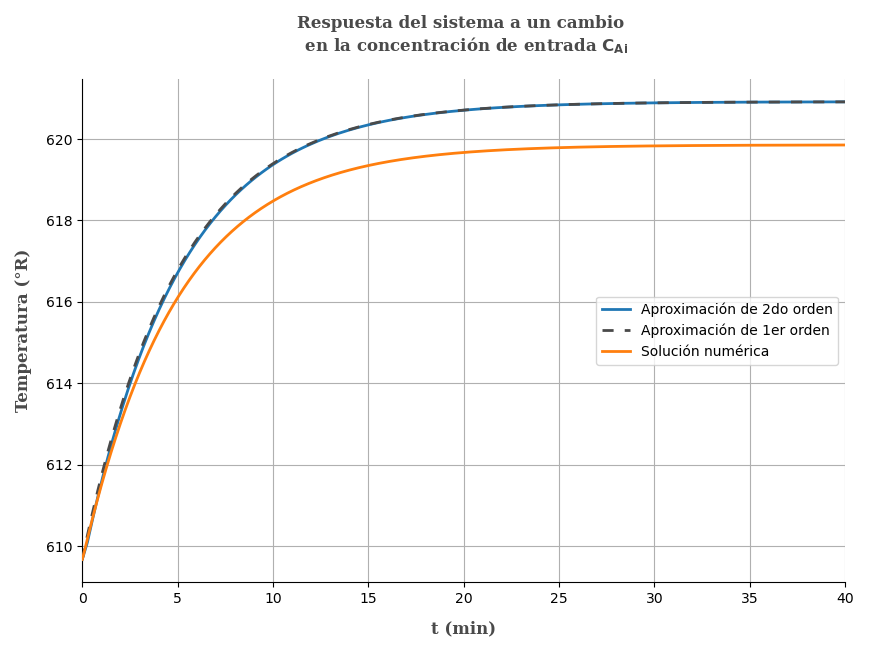
\includegraphics{././images/p5.21-seborg/p521r.png}

}

\caption{Solución gráfica p5.21}

\end{figure}

Como se observa en la gráfica una aproximación de primer orden es
suficiente, notesé también que existen una sobreestimación de la
ganancia con la aproximación que se ha realizado.

\hypertarget{referencias-10}{%
\section{Referencias}\label{referencias-10}}

\begin{itemize}
\tightlist
\item
  Seborg, D. E.; Edgar, T. F.; Mellichamp, D. A.; Doyle, F. J. (2016).
  \emph{Process Dynamics and Control} (4th edition). John Wiley \& Sons,
  Inc.~ISBN 978-1-119-28591-5.
\end{itemize}

\part{Sistemas físicos de segundo orden}

\hypertarget{dos-reactores-en-serie-con-un-perturbaciuxf3n-tipo-impulso-unitario}{%
\chapter{Dos reactores en serie con un perturbación tipo impulso
unitario}\label{dos-reactores-en-serie-con-un-perturbaciuxf3n-tipo-impulso-unitario}}

\begin{figure}

{\centering 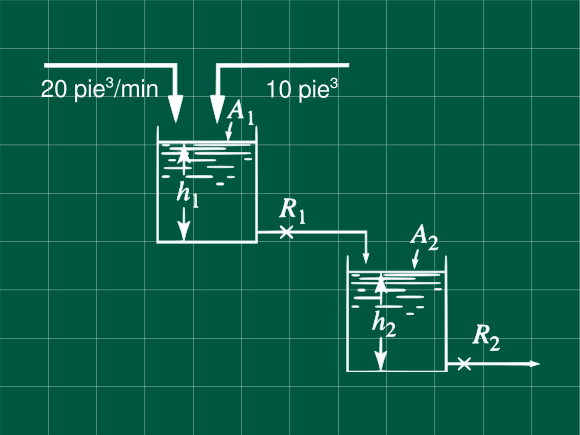
\includegraphics{././images/p7.2-coughanowr/headercontrol72.png}

}

\caption{diagrama p7.2}

\end{figure}

Dos tanques mostrados en la figura, operan en estado estacionario. At
t=0 se agregan al primer tanque, 10 pie³ de agua de manera repentina.
Usando apropiadamente las figuras y ecuaciones, determine la máxima
desviación del nivel del líquido en ambos tanques del estado
estacionario y el tiempo en el cuál ocurre.

\[
\begin{array}{l}
A_1=A_2=10\space pie²\\
R_1=0.1\space pie/(pie³/min)\\
R_2=0.35\space pie/(pie³/min)\\
\end{array}
\]

Escribiendo las ecuaciones de balance

\hypertarget{obtenciuxf3n-de-la-ecuaciuxf3n-en-transferencia-1}{%
\subsection{Obtención de la ecuación en
transferencia}\label{obtenciuxf3n-de-la-ecuaciuxf3n-en-transferencia-1}}

Pero \(q_1 = h_1/R_1\) y \(dV_1 = A_1dh_1\)

\[
q- \frac{h_1}{R} = A\frac{dh_1}{dt} \space\space\space\space (1)
\]

Escribiendo el balance en estado estacionario

\[
q_s- \frac{h_{1s}}{R_1} = 0 \space\space\space\space (2)
\]

Restando (1) con (2) para obtener las variables desviación y recordando
que \(dh=d(h-h_s)\), por ser \(h_s\) constante.

\[
q-q_s-\frac{h_1-h_{1s}}{R_1}=A\frac{d(h_1-h_{1s})}{dt}
\]

\[
Q - \frac{H_1}{R_1} = A\frac{dH_1}{dt}
\]

Aplicando la tranformada de Laplacey sabiendo que
\(H_1(t=0)= h_1-h_{1s}=h_{1s}-h_{1s}=0\)

\[
Q(s) - \frac{H_1(s)}{R_1} = A_1\left[sH_1(s)-H_1(t=0)\right]\\
\]

\[
Q(s) - \frac{H_1(s)}{R_1} = A_1sH_1(s)
\]

Reordenando obtenemos la ecuación de tranferencia del primer tanque

\[
\frac{H_1(s)}{Q(s)} = \frac{R_1}{A_1R_1s+1}\space\space\space\space\textbf{... (3)}
\]

Reemplazando datos \(R_1=0.1\text{   ;}A_1=10\) obtenemos la ecuación de
tranferencia del primer tanque.

\[
\mathbf{\frac{H_1(s)}{Q(s)} = \frac{0.1}{1s+1}} \space\space\space\space\textbf{... }\mathbf{(\alpha)}
\]

De similar manera podemos obtener la ecuación de transferencia para el
segundo tanque

\[
\frac{H_2(s)}{Q_1(s)} = \frac{R_2}{A_2R_2s+1}\space\space\space\space\textbf{... (4)}
\]

Recuerde que tambien se cumple \[
Q_1(s)=\frac{H_1(s)}{R_1}
\]

Reemplazando en (4)

\[
\frac{H_2(s)\cdot R_1}{H_1(s)} = \frac{R_2}{A_2R_2s+1}\space\space\space\space\textbf{... (5)}
\]

Multipicando las ecuaciónes (3) con (5) y simplificando obtenemos la
ecuación de transferencia del segundo tanque.

\[
\frac{H_2(s)}{Q(s)} = \frac{R_2}{(A_2R_2s+1)(A_1R_1s+1)}\space\space\space\space\textbf{... (6)}
\]

Reemplazando con los datos
\(R_1=0.1\text{   ;}A_1=A_2=10\text{   ;}R_2=0.35\)

\[
\mathbf{\frac{H_2(s)}{Q(s)} = \frac{0.35}{(3.5s+1)(s+1)}} \space\space\space\space\textbf{... }\mathbf{(\beta)}
\]

Ahora describamos la perturbación

\[
Q(t)=
\begin{cases}
   0 \space &\text{si } t<0\\
   10 \space\ pie³/min \space\space\space (\infty)&\text{si } t=0 \space min\\
   0 \space\ &\text{si } t>0 \\
\end{cases}
\]

Entonces \[
Q(t) = 10 \delta (t)
\]

Aplicando la transformada

\[
Q(s) = 10
\]

Para el primer tanque reemplazanado en la ecuación \((\alpha)\)

\[
H_1(s) = \frac{0.1Q(s)}{s+1}  = \frac{0.1\times 10}{s+1} =\frac{1}{s+1} 
\]

Antitransformando

\[
H_1(t) = e^{-t}
\] Notamos que la función es decreciente el máximo valor que toma es al
inicio. Por lo que el máximo valor de la desviación es cuando t=0. Puede
confirmar esto reemplazando cualquier valor de t\textgreater0, ó
graficando la función.

\[
H_1(t=0) = e^{-0} = 1
\]

Entonces el la desviación máxima es \textbf{1 pie} en el nivel del
líquido del primer tanque a \textbf{t = 0 min}.

Para el segundo tanque reemplazando \(Q(s)=10\) en la ecuación \(\beta\)

\[
H_2(s) = \frac{0.35\times Q(s)}{(3.5s+1)(s+1)} = \frac{3.5}{(3.5s+1)(s+1)}
\]

Expandiendo el termino del lado derecho en fracciones parciales (Puede
obtener el mismo resultado si usa las tablas)

\[
\frac{3.5}{(3.5s+1)(s+1)} = \frac{A}{(3.5s+1)}+\frac{B}{(s+1)}
\]

\[
3.5 = A(s+1)+B(3.5s+1)
\]

Recuerde que es una ecuación y cumple para cualquier valor de \(s\).
Eligiendo el valor conveniente de \(s\) podemos hallar las constantes.

Cuando \(s=-1\) entonces \(B = -0.35/2.5\)

para \(s=-1/3.5\) el valor \(A=0.35\times 3.5/2.5\)

En nuestra ecuación original y reorganizando para la antitransformada

\[
H_2(s)=\frac{0.35}{2.5}\left(\frac{1}{s+1/3.5}-\frac{1}{s+1}\right)
\]

Aplicando la transformada inversa

\[
H_2(t)=\frac{0.35}{2.5}\left(e^{-t/3.5}-e^{-t}\right)
\]

Derivando e igualando a cero para hallar el máximo.

\[
\frac{dH_2(t)}{dt}=\frac{0.35}{2.5}\left(-\frac{e^{-t/3.5}}{3.5}-(-1)e^{-t}\right)=0
\]

Operando

\[
3.5e^{-t}=e^{-t/3.5}
\]

Despejando t

\[
t=\frac{3.5\times ln(3.5)}{2.5} = 1.7539\text{ min}
\]

Reemplazandoen H\_2(t) \[
H_2(t=1.7539)=\frac{0.35}{2.5}\left(e^{-1.7539/3.5}-e^{-1.7539}\right) = 0.0606\text{ pie}
\]

Entonces la máxima desviación para el segundo tanque se da cuando
\textbf{t = 1.7539 min} con una desviación del nivel del líquido de
\textbf{0.0606 pie}.

\emph{Nótese que no se nos pide hallar el nivel del liquido (h) cuando
la desviación es máxima si no solamente la desviación máxima (H). Si se
quisiera hallar el nivel del liquido utilice la ecuación
\emph{\(H(t) = h(t)-h_s\)} y despeje \(h_s\) de las ecuaciones del
balance en estado estacionario.}

Es interesante analizar los estados de este sistema mediante gráficos,
así que lo incluyo por si alguien desea verlo.

\begin{figure}

{\centering 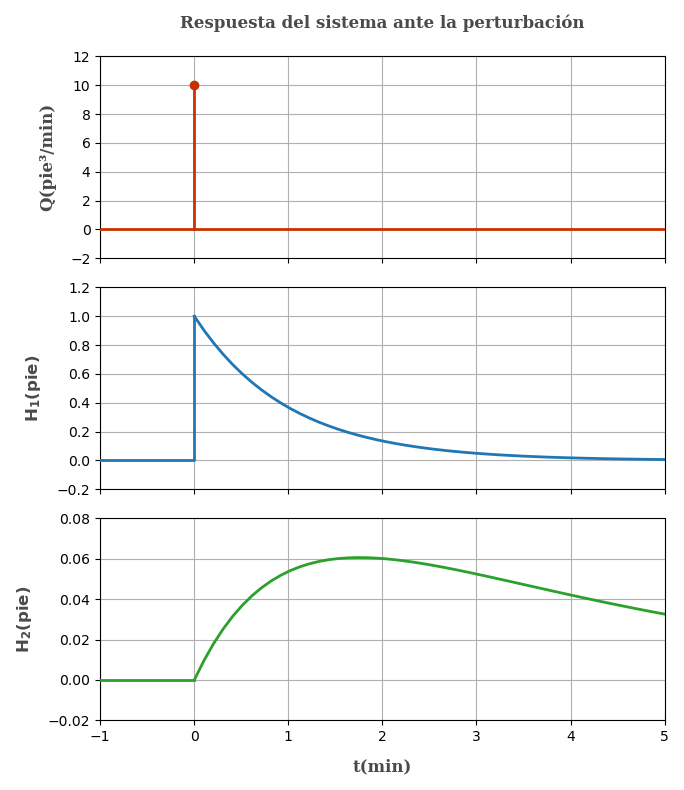
\includegraphics{././images/p7.2-coughanowr/p72r.png}

}

\caption{respuesta del sistema p7.2}

\end{figure}

\hypertarget{referencias-11}{%
\section{Referencias}\label{referencias-11}}

\begin{itemize}
\tightlist
\item
  Coughanowr, D. R.; LeBlanc, S. E. (2009). \emph{Process Systems
  Analysis and Control} (3rd edition). McGraw-Hill. ISBN
  978-0-07-339789-4.
\end{itemize}

\hypertarget{reactores-en-serie-con-una-respuesta-cruxedticamente-amortiguada}{%
\chapter{Reactores en serie con una respuesta críticamente
amortiguada}\label{reactores-en-serie-con-una-respuesta-cruxedticamente-amortiguada}}

\begin{figure}

{\centering 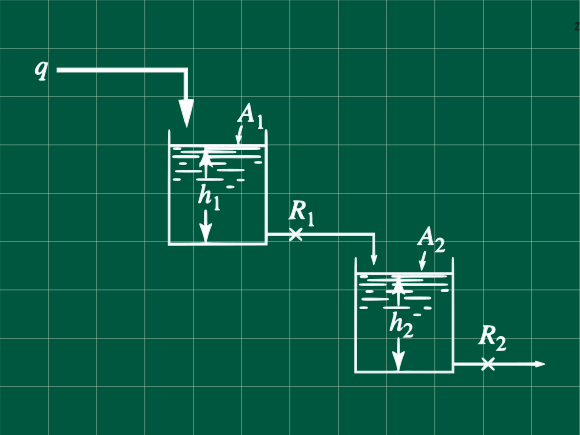
\includegraphics{././images/p7.3-coughanowr/headercontrol73.png}

}

\caption{diagrama p7.3}

\end{figure}

El sistema de tanques mostrado en la figura, opera en estado
estacionario, cuando un cambio en el caudal tipo paso unitario o
heaviside ocurre en el caudal de ingreso del primer tanque. La respuesta
de la altura del segundo tanque es críticamente amortiguada, y toma 1
min en el cambio del nivel en llegar al 50 \% de su cambio total.

Si la razón de las áreas seccionales es \(A_1/A_2 = 2\) calcular la
razón \(R_1/R_2\). Calcule la constante de tiempo para ambos tanques.
¿Cuanto tiempo le toma al primer tanque llegar al 90\% de su cambio
total?

\hypertarget{resoluciuxf3n-2}{%
\section{Resolución}\label{resoluciuxf3n-2}}

Escribamos las ecuaciones de transferencia de cada tanque. Aquí
pondremos directamente las ecuaciones de transferencia, las cuales ya
han sido deducidas en los anteriores problemas.

Para el primer tanque tenemos \[
\frac{H_1(s)}{Q(s)}=\frac{R_1}{A_1R_1s+1}\space\space\space\space\textbf{ ... (1)}
\]

Para el segundo tanque

\[
\frac{H_2(s)}{Q_1(s)}=\frac{R_2}{A_2R_2s+1}\space\space\space\space\textbf{ ... (2)}
\]

Pero sabemos que:

\[
Q_1(s) = \frac{H_1(s)}{R_1}
\]

Reemplazando en (2)

\[
\frac{H_2(s)R_1}{H_1(s)}=\frac{R_2}{A_2R_2s+1}\space\space\space\space\textbf{ ... (3)}
\]

Multiplicando (3) y (1)

\[
\frac{H_2(s)}{Q(s)}=\frac{R_2}{(A_2R_2s+1)(A_1R_1s+1)}
\]

haciendo \(\tau_1 = A_1R_1\) y \(\tau_2=A_2R_2\)

\[
\frac{H_2(s)}{Q(s)}=\frac{R_2}{(\tau_2s+1)(\tau_1s+1)}\space\space\space\space\textbf{ ... (4)}
\]

Operando para compararlo con un modelo de sistema de segundo orden

\[
\frac{H_2(s)}{Q(s)}=\frac{R_2}{\tau_1\tau_2+(\tau_1+\tau_2)s+1}
\]

Comparando con un sistema de segundo orden

\[
\frac{Y(s)}{X(s)}=\frac{1}{\tau^2 s^2+2\zeta\tau s+1}
\]

\[
\begin{array}{ll}
\zeta<1 & \text{Subamortiguado u oscilatorio}\\
\zeta=1 & \text{Críticamente amortiguado}\\
\zeta>1 & \text{Sobreamortiguado o no oscilatorio}\\
\end{array}
\]

Cuando \(\zeta=1\) sabemos que las raices son iguales, es decir para la
ecuación (4) las constantes de tiempo son iguales para ambos tanques,
pero igual operaremos para demostrarlo.

Comparando los denominadores de las dos anteriores ecuaciones con
\(\zeta=1\) tenemos

\[
\tau_1+\tau_2=2\zeta\tau=2\tau\\
\tau^2=\tau_1\tau_2
\]

Operando

\[
(\tau_1-\tau_2)^2=0
\]

De donde se deduce que \(\tau_1=\tau_2=\tau\)

Con esta igualda deducimos la relación \(R_1/R_2\)

\[
\tau_1=\tau_2\\
A_1R_1=A_2R_2
\]

\[
\frac{A_1}{A_2}=2=\frac{R_2}{R_1}
\]

\[
\mathbf{R_1/R_2=1/2}
\]

Del enunciado, se nos indica que hay un cambio en el caudal de
entrada(un cambio tipo escalón unitario), esto es con M como la magnitud
del cambio:

\[
Q(s)=\frac{M}{s}
\]

Reemplazando en la ecuación (4) y sabiendo que \(\tau_1=\tau_2=\tau\)

\[
H_2(s)=\frac{M}{s}\frac{R_2}{(\tau s+1)^2}\space\space\space\space\textbf{... (5)}
\]

Expandiendo el segundo miembro de la ecuacióne en fracciones parciales
(Nota: tambien puede usar tablas para hallar la transformada
directamente)

\[
\frac{1}{s(\tau s+1)^2}=\frac{A}{s}+\frac{B}{\tau s+1}+\frac{C}{(\tau s+1)^2}
\]

Operando

\[
1=A(\tau s+1)^2+Bs(\tau s+1)+Cs\space\space\space\space\textbf{... }\mathbf{\alpha}
\]

Seleccionando \(s\) apropiadamente

Para \(s = 0\), \(A =1\)

Para \(s=-1/\tau\), \(C=-\tau\)

Operando \(\alpha\) para hallar \(B\)

\[
0s^2+0s+1=(B\tau+\tau^2)s^2+(2\tau+B+C)s+1
\]

Comparando los terminos que acompañan a \(s^2\) determinamos que
\(B=-\tau\)

Reemplazando A, B y C en nuestra ecuación (5) expresada con fracciones
parciales.

\[
H_2(s)=MR_2\left(=\frac{1}{s}-\frac{\tau}{\tau s+1}-\frac{\tau}{(\tau s+1)^2}\right)
\]

Aplicando la antitransformada de Laplace y operando

\[
H_2(t) = MR_2\left[1-\left(1+\frac{t}{\tau}\right)e^{-t/\tau}\right]
\]

Para hallar el cambio total hacemos que \(t\to\infty\), hallamos que
\(H_2(t\to\infty)=MR_2\)

Del enunciado nos indican que para cuando t = 1, el tanque dos alcanza
50\% de su cambio total. Reemplazando ese dato tenemos
\(\big[t=1,H(t=1)=0.5MR_2\big]\):

\[
0.5\cdot MR_2 = MR_2\left[1-\left(1+\frac{1}{\tau}\right)e^{-1/\tau}\right]
\]

Simplificando

\[
\frac{1}{2}=\left(1-\frac{1}{\tau}\right)e^{-1/\tau}\space\space\space\space\textbf{... }\mathbf{\beta}
\]

Usemos la expansión en series de Taylor truncada de primer orden.

\[
f(x)=f(x_0)+f'(x_0)(x-x_0)
\]

Aplicada a la función \(f(x)=e^{-x}\) con \(x_0=0\) se tiene:

\[
e^{-x}=e^{-0}-e^{-0}(x-0)
\]

\[
e^{-x}=1-x
\]

Para \(-x=-1/\tau\)

\[
e^{-1/\tau}=1-\frac{1}{\tau}
\]

Reemplazando en el ecuación \(\beta\)

\[
\frac{1}{2}=\left(1-\frac{1}{\tau}\right)^2
\]

Despejando y recordando que el \(\sqrt{x^2}=|x|\)

\[
\tau=\frac{\sqrt{2}}{\sqrt{2} ± 1}
\]

Obtenemos dos soluciones \[
\begin{array}{ll}
\tau_a=0.58578 & \tau_b=3.41421\\
\end{array}
\]

Para escoger un valor de \(\tau\) reemplazamos en la ecuación original y
aquel que nos dé una aproximación mejor sera escogida

Reemplazando \(\tau=\tau_a=0.58578\) en la ecuación \(\beta\) \[
0.5\approx -0.12826
\]

Para \(\tau=\tau_b=3.41421\) en la ecuación \(\beta\)

\[
0.5\approx 0.5276
\]

Entonces nuestra constante de tiempo para ambos tanques es
\(\mathbf{\tau_1=\tau_2=3.41421}\)

\emph{Nota: Si desea una valor exacto de la solución para \(\tau\) puede
usar métodos númericos como el de \textbf{Newton-Raphson}, pero como
incluso las funciones tranferencia son simplemente aproximaciones de un
sistema real, no tiene mucho sentido usar valores exactos para la
solución de funciones aproximadas, pues estas como sun nombre indica son
\textbf{funciones aproximadas}.}

Para saber a que tiempo el tanque 1 alcanza 90 \% de su cambio total
cuando \(Q(s) = M/s\) y \(\tau = A_1R_1\) operamos en la ecuación (1)

\[
H_1(s)=\frac{MR_1}{s(\tau s +1)}
\]

\[
H_1(s)=MR_1\left(\frac{1+\tau s - \tau s}{s(\tau s +1)}\right)
\]

\[
H_1(s)=MR_1\left(\frac{1}{s}-\frac{1}{s+1/\tau}\right)
\]

Aplicando la antitransformada

\[
H_1(t)=MR_1\left(1-e^{-t/\tau}\right)
\]

Sabemos que cuando \(H_1(t\to\infty)=MR_1\) corresponde al cambio total.
Nos piden hallar \(t_{90\%}\) sabiendo que \(H(t_{90\%})= 0.9MR_1\).
Reemplazando en la ecuación anterior

\[
0.9MR_1=MR_1\left(1-e^{-t_{90\%}/\tau}\right)
\]

\[
t_{90\%}=\frac{ln(10)}{\tau}
\]

\[
\mathbf{t_{90\%}=0.6744 \textbf{ min}}
\]

\hypertarget{referencias-12}{%
\section{Referencias}\label{referencias-12}}

\begin{itemize}
\tightlist
\item
  Coughanowr, D. R.; LeBlanc, S. E. (2009). \emph{Process Systems
  Analysis and Control} (3rd edition). McGraw-Hill. ISBN
  978-0-07-339789-4.
\end{itemize}



\end{document}
